\documentclass[CJK,aspectratio=169]{beamer}  %aspectratio控制页面的宽高比,16:9充满屏幕
\usepackage{beamerthemesplit}
\usetheme{Warsaw}
\usepackage{ctex} %中文字体设置
\usepackage{subfig}
\usepackage{amssymb,amsmath,mathtools}
\usepackage{amsfonts,booktabs}
\usepackage{lmodern,textcomp}
\usepackage{color}
\usepackage{tikz}
%\usepackage[latin1]{inputenc}
\usepackage{natbib}
\usepackage{bbding}
\usepackage{multicol}
\usepackage{caption} 
\usepackage{graphicx}
\usepackage{makecell}                 % 三线表-竖线
\usepackage{booktabs}                 % 三线表-短细横线

\begin{document}
	
	\title{开题答辩}
	\author[顾睿 (LZU)]{顾睿 \inst{1}}
	\institute[*]{\inst{1} 兰州大学,信息科学与工程学院\\
		npukujui11@gmail.com}
	
	\newcommand{\monthname}[1][\the\month]{%
		\ifcase#1\or
		1\or 2\or 3\or 4\or 5\or 6\or 7\or 8\or 9\or 10\or 11\or 12\fi}
		
	\renewcommand{\today}{\the\year 年 \monthname[\the\month] 月 \the\day 日}
	\renewcommand{\figurename}{\tiny 图}
	\renewcommand{\tablename}{表}
	\renewcommand{\refname}{References}
	\date{\today}
	
	\begin{frame}
		\titlepage
	\end{frame}
	
	\begin{frame}
		\begin{multicols}{2}
			\small \tableofcontents
		\end{multicols}
	\end{frame}
	
%	\begin{frame} \transblindshorizontal<1>  %百叶窗效果
%		
%		\begin{itemize}
%			\item <1> {\bf 章节4}
%			\begin{itemize}
%				\item {章节4.1}
%				\begin{itemize}
%					\item {4.1.2}
%				\end{itemize}
%			\end{itemize}
%			
%		\end{itemize}		
%	\end{frame}
	
	\section{研究介绍}
	
	\subsection{研究意义}
	
	\begin{frame}
	{\zihao{-4} \yahei \textbf{弱光图像增强}}
	
	\vspace{0.1cm}

	{\zihao{-6} \yahei \textbf{弱光图像增强}旨在从黑暗和噪声图像中恢复正常光线和无噪声图像,这是一个长期存在的重要计算机视觉课题。在硬件条件不变的情况下,给定降质图像或恶劣天气下拍摄的图像,研究生成高质量、无噪声图像等增强方法,在实际应用中非常有意义。}

		%它具有广泛的应用领域,包括视频监控,自动驾驶和计算摄影方面。特别是,智能手机摄影已经变得无处不在。受限于相机光圈的大小、实时处理的要求以及存储器的约束,在昏暗环境中用智能手机的相机拍摄照片尤其具有挑战性。
		
	\begin{figure}
		\centering
		\setlength{\abovecaptionskip}{-0.15cm}
		\begin{minipage}{.08\paperwidth}
			\centering
			\setlength{\abovecaptionskip}{-0.45cm}
			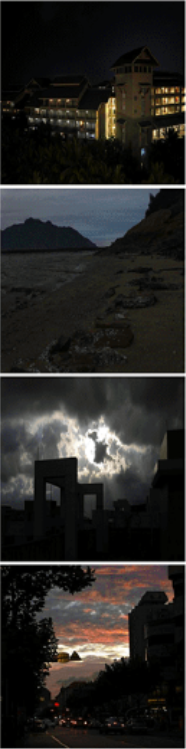
\includegraphics[width=\linewidth]{picture/LLIE/LightingNet/LOW}
			\label{fig: LOW}
			\caption*{\tiny LOW}
		\end{minipage}
		\begin{minipage}{.08\paperwidth}
			\centering
			\setlength{\abovecaptionskip}{-0.45cm}
			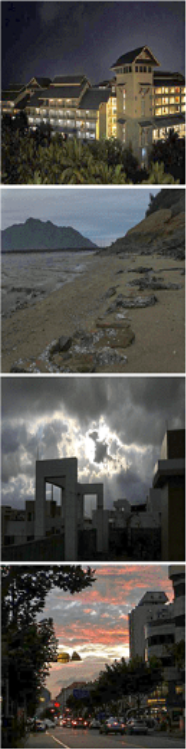
\includegraphics[width=\linewidth]{picture/LLIE/LightingNet/BIMEF}
			\label{fig: BIMEF}	
			\caption*{\tiny BIMEF}
		\end{minipage}
		\begin{minipage}{.08\paperwidth}
			\centering
			\setlength{\abovecaptionskip}{-0.45cm}
			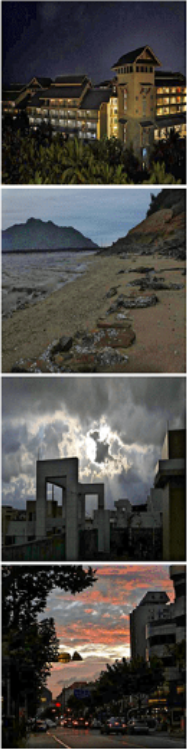
\includegraphics[width=\linewidth]{picture/LLIE/LightingNet/NPE}
			\label{fig: NPE}	
			\caption*{\tiny NPE}
		\end{minipage}
		\begin{minipage}{.08\paperwidth}
			\centering
			\setlength{\abovecaptionskip}{-0.45cm}
			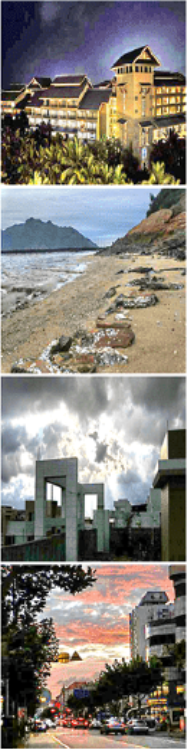
\includegraphics[width=\linewidth]{picture/LLIE/LightingNet/LIME}
			\label{fig: LIME}	
			\caption*{\tiny LIME}
		\end{minipage}
		\begin{minipage}{.08\paperwidth}
			\centering
			\setlength{\abovecaptionskip}{-0.45cm}
			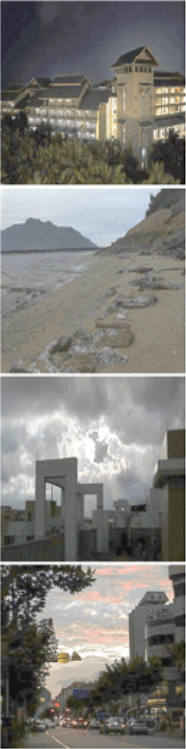
\includegraphics[width=\linewidth]{picture/LLIE/LightingNet/LTC}
			\label{fig: LTC}	
			\caption*{\tiny LTC}
		\end{minipage}
		\begin{minipage}{.08\paperwidth}
			\centering
			\setlength{\abovecaptionskip}{-0.45cm}
			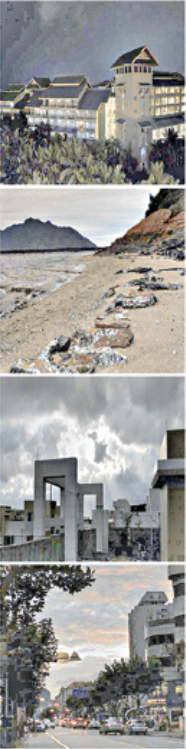
\includegraphics[width=\linewidth]{picture/LLIE/LightingNet/MSR}
			\label{fig: MSR}	
			\caption*{\tiny MSR}
		\end{minipage}
		\begin{minipage}{.08\paperwidth}
			\centering
			\setlength{\abovecaptionskip}{-0.45cm}
			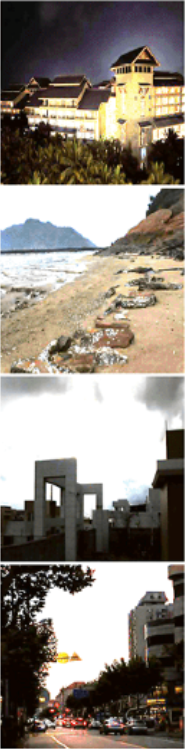
\includegraphics[width=\linewidth]{picture/LLIE/LightingNet/RUAS}
			\label{fig: RUAS}	
			\caption*{\tiny RUAS}
		\end{minipage}
		\begin{minipage}{.08\paperwidth}
			\centering
			\setlength{\abovecaptionskip}{-0.45cm}
			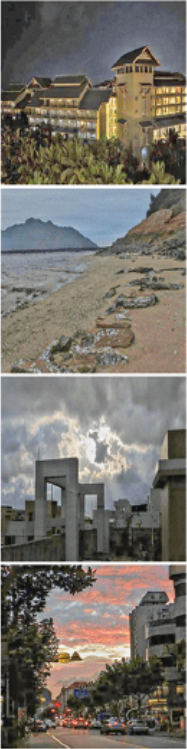
\includegraphics[width=\linewidth]{picture/LLIE/LightingNet/TBEFN}
			\label{fig: TBEFN}	
			\caption*{\tiny TBEFN}
		\end{minipage}
		\begin{minipage}{.08\paperwidth}
			\centering
			\setlength{\abovecaptionskip}{-0.45cm}
			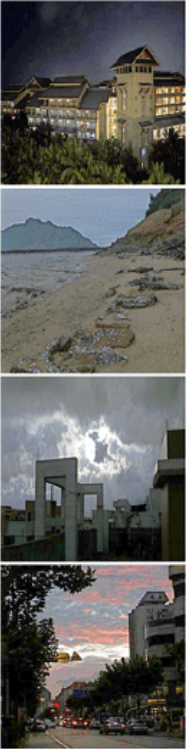
\includegraphics[width=\linewidth]{picture/LLIE/LightingNet/ZERO-DCE}
			\label{fig: ZERO-DCE}	
			\caption*{\tiny ZERO-DCE}
		\end{minipage}
		\begin{minipage}{.08\paperwidth}
			\centering
			\setlength{\abovecaptionskip}{-0.45cm}
			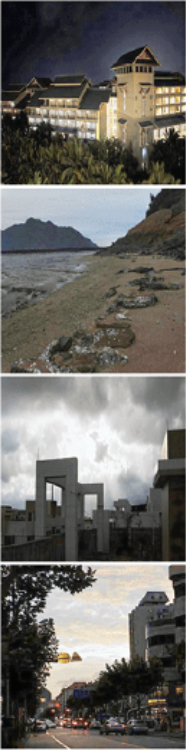
\includegraphics[width=\linewidth]{picture/LLIE/LightingNet/LightingNet}
			\label{fig: LightingNet}	
			\caption*{\tiny LightingNet}
		\end{minipage}
		\captionsetup{font=scriptsize}
%		\caption{
%			\label{fig: LLIE}
%			弱光图像增强
%		}
	\end{figure}
		
	\end{frame}
	
	\begin{frame}
		{\zihao{-4} \yahei \textbf{研究意义}}
		\begin{figure}
			\centering			
			\begin{minipage}{.4\columnwidth}
				%\centering
				%\small
				\begin{itemize}
					\item \zihao{-5} \yahei \textbf{应用领域}
					
					\item[\checkmark]
					\zihao{-5} \yahei 视频监控\textcolor{blue}{\citep{s20020495}}
					
					% 视频监控设备作为安防系统的输人终端,提供了最基础的案件复原、实时监控的素材,在案情预防、分析和侦破等方面发挥着非常重要的作用。然而,实际场景的监控视频质量却往往与侦查机关的案件侦察办理需求之间存在差距。一方面,实地部署的摄像头硬件的成像条件有限;另一方面,为了控制存储空间和传输成本,监控视频往往使用较低的码率进行压缩存储,导致视频中很多细节的丢失。许多对破案有意义的视频信息,在压缩存储和传输的过程中遭到丢失。这时利用低质图像、视频复原技术,能够将低质量的监控视频增强为高质量的目标视烦,便于进一步进行人工分析或后续的自动识别;也可通过对感兴趣区域进行跟踪和放大,对人脸、行人或车牌等进行识别。
					
					% 随着智慧城市的不断发展,室外监控逐渐覆盖公共生活的方方面面。然而,由于室外拍摄环境较为复杂,监控视频会受到各种各样降质因素的影响,比如雨天拍摄的视频中雨点对背景的遮挡、大雾天气下能见度的降低、低光照环境下大量物体信号的丢失、雨雾环境下大量物体细节的丢失等。这些因素对后续的人工分析和计算机视觉应用造成了障得。而使用低质图像、视频重建技术对这些因素进行移除,能够提升图像、视频的能见度,增强高频细节,便于后续处理与分析。对雨天图像进行雨痕去除,能够提升图像的视觉质量,并使图像识别结果变得正确。
					
					
					\item[\checkmark]
					\zihao{-5} \yahei 自动驾驶\textcolor{blue}{\citep{li2021deep}}
					
					\item[\checkmark]
					\zihao{-5} \yahei 计算摄影\textcolor{blue}{\citep{ma2022toward}}
					
					\item[\checkmark]
					\zihao{-5} \yahei ......
					
				\end{itemize}
			\end{minipage}
			\begin{minipage}{.55\columnwidth}
				\setlength{\abovecaptionskip}{-0.05cm}
				\centering
				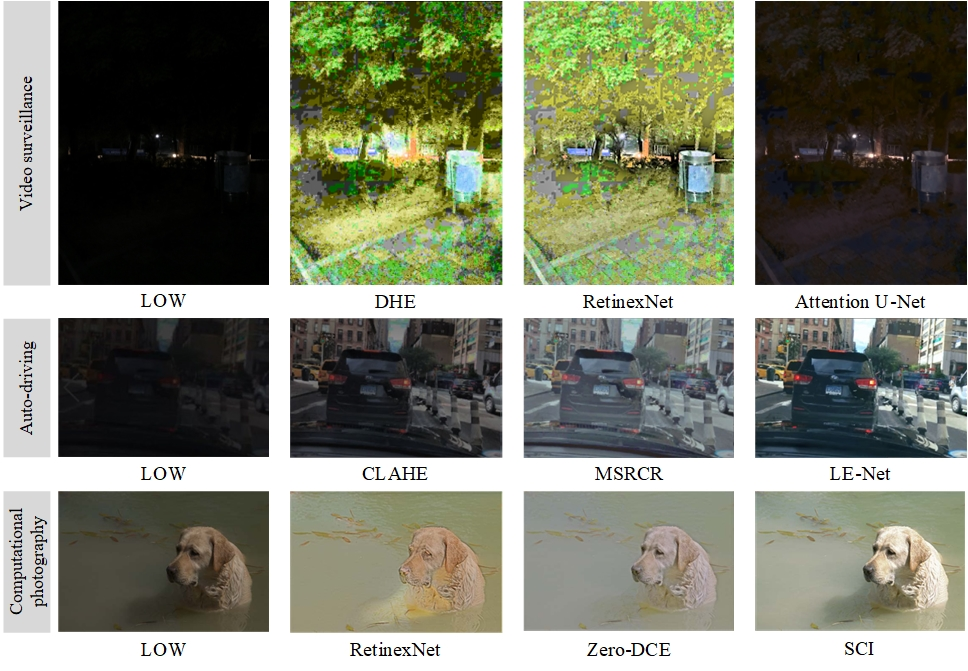
\includegraphics[width=\linewidth]{picture/LLIE/application scenarios}
				\caption{
					\label{fig: application scenarios}
					\tiny Application scenarios.
				}
			\end{minipage}
		\end{figure}
	\end{frame}
	
	\begin{frame}
		{\zihao{-4} \yahei \textbf{研究意义}}
		
		\vspace{0.1cm}
		
		{\zihao{-6} \yahei 基于软件技术的图像复原增强技术得到了广泛研究,其通过引入外部信息、加入先验、基于大数据集进行学习等方式,将输入的弱光图像的低光细节复原,产生接近降质前理想质量的低噪图。}

		\begin{figure}
			\centering			
			\begin{minipage}{.4\columnwidth}
				\begin{itemize} 
					\item \zihao{-5} \yahei \textbf{挑战}
					
					% 传统方法包括基于直方图均衡的方法和基于 Retinex 模型的方法。
					\zihao{6} \yahei 伪影(Artifacts)
					
					\zihao{6} \yahei 色差(Color Deviations) 
					% 传统方法一般通过有效的先验或正则化来解决噪声问题。但是寻找到有效的先验和正则化相当具有挑战性,不正确的先验或正则化可能导致增强结果中的伪像和颜色偏差。
					
					\zihao{6} \yahei 噪声(Noise)
					% 但是这些方法存在一些局限性,例如在 Retinex 模型中通常忽略噪声,因此在增强结果中保留或放大噪声;
					
					\zihao{6} \yahei 鲁棒性(Robustness)
					% 但是现有的低光照图像增强技术聚焦于构建数据驱动的深度网络,通常其网络模型复杂,导致计算效率低、推理速度慢,并且由于对于训练数据分布的依赖性导致其在未知场景下的性能缺乏保障。
					% 物体边缘不清晰时,像素级损失往往会模糊边缘,破坏图像细节。
					
					\zihao{6} \yahei 边缘细节(Edge Details)
					% 现有的方法可能无法在极暗或极明亮的区域恢复图像的边缘细节。				
				\end{itemize}
			\end{minipage}
			\begin{minipage}{.58\columnwidth}
				\setlength{\abovecaptionskip}{-0.05cm}
				\centering 
				\begin{minipage}{0.17\columnwidth}
					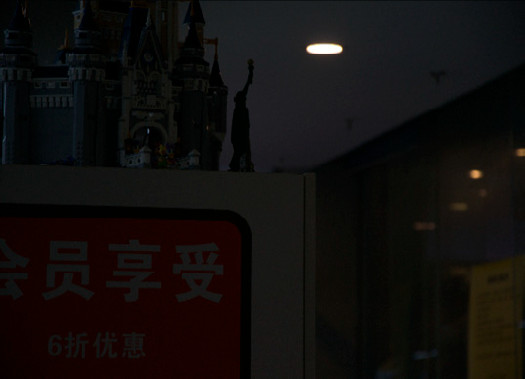
\includegraphics[width=\linewidth]{picture/LLIE/VE-LOL-L/input}
					\caption*{\tiny input \\ \quad }
					\label{fig: input}
				\end{minipage}
				\begin{minipage}{0.17\columnwidth}
					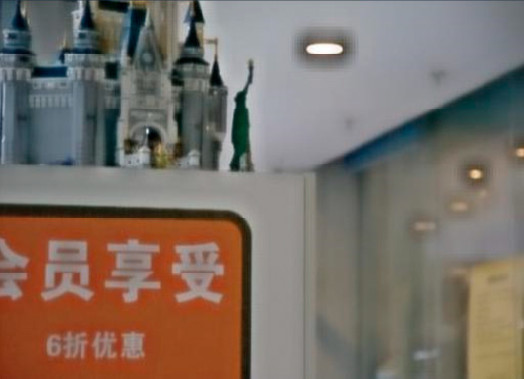
\includegraphics[width=\linewidth]{picture/LLIE/VE-LOL-L/LLNet}
					\caption*{\tiny LLNet \\ (2017)}
					\label{fig: LLNet}	
				\end{minipage}
				\begin{minipage}{0.17\columnwidth}
					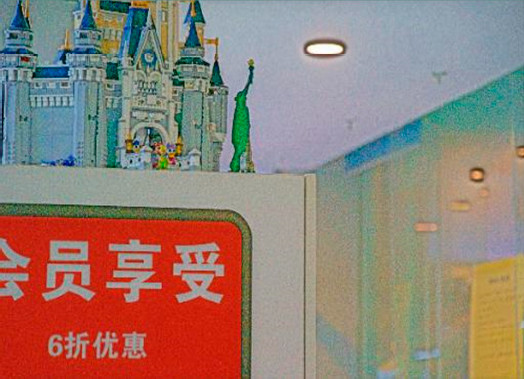
\includegraphics[width=\linewidth]{picture/LLIE/VE-LOL-L/RetinexNet}
					\caption*{\tiny RetinexNet \\ (2018)}
					\label{fig: RetinexNet_LOL}	
				\end{minipage}
				\begin{minipage}{0.17\columnwidth}
					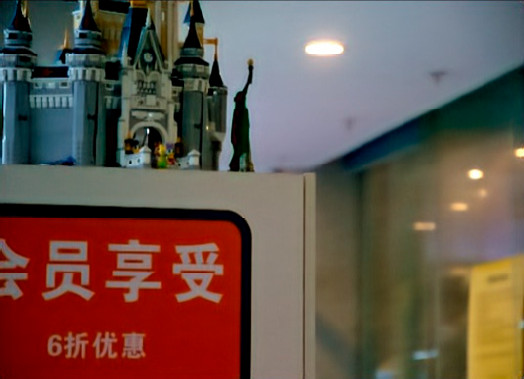
\includegraphics[width=\linewidth]{picture/LLIE/VE-LOL-L/MBLLEN}
					\caption*{\tiny MBLLEN \\ (2018)}
					\label{fig: MBLLEN_LOL}	
				\end{minipage}
				\begin{minipage}{0.17\columnwidth}
					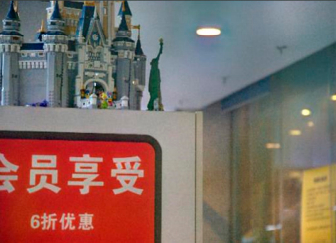
\includegraphics[width=\linewidth]{picture/LLIE/VE-LOL-L/EnlightenGAN}
					\caption*{\tiny EnlightenGAN \\ (2019)}
					\label{fig: EnlightenGAN}	
				\end{minipage}
				\begin{minipage}{0.17\columnwidth}
					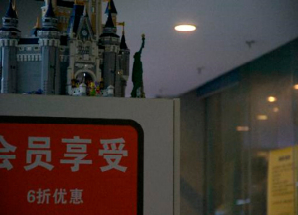
\includegraphics[width=\linewidth]{picture/LLIE/VE-LOL-L/RRDNet}
					\caption*{\tiny RRDNet \\ (2020)}
					\label{fig: RRDNet}	
				\end{minipage}
				\begin{minipage}{0.17\columnwidth}
					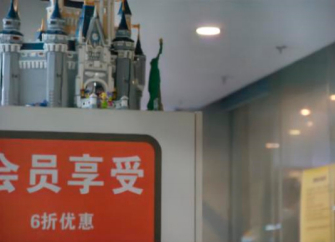
\includegraphics[width=\linewidth]{picture/LLIE/VE-LOL-L/DRBN}
					\caption*{\tiny DRBN \\ (2020)}
					\label{fig: DRBN}	
				\end{minipage}
				\begin{minipage}{0.17\columnwidth}
					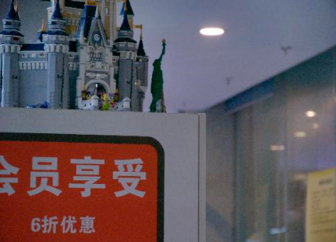
\includegraphics[width=\linewidth]{picture/LLIE/VE-LOL-L/Zero-DCE++}
					\caption*{\tiny Zero-DCE++ \\ (2021)}
					\label{fig: Zero-DCE++}	
				\end{minipage}
				\begin{minipage}{0.17\columnwidth}
					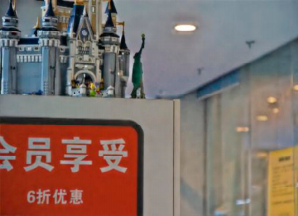
\includegraphics[width=\linewidth]{picture/LLIE/VE-LOL-L/KinD++}
					\caption*{\tiny KinD++ \\ (2021)}
					\label{fig: KinD++}	
				\end{minipage}
				\begin{minipage}{0.17\columnwidth}
					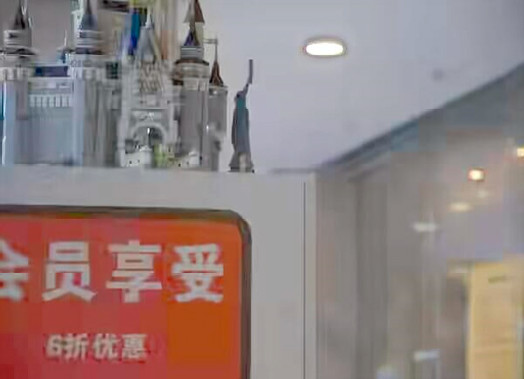
\includegraphics[width=\linewidth]{picture/LLIE/VE-LOL-L/URetinexNet}
					\caption*{\tiny URetinexNet \\ (2022)}
					\label{fig: URetinexNet}	
				\end{minipage}
				
				%\captionsetup{font=scriptsize}
				\caption{
					\label{fig: VE-LOL-L Visual} 
					\tiny Visual results of different algorithms on low-illumination images sampled from the VE-LOL-L dataset.
				}
			\end{minipage}
		\end{figure}
	\end{frame}
	
	\subsection{研究背景和现状}
	
	\subsubsection{传统弱光图像增强方法}
	
	\begin{frame}
		{\zihao{-5} \yahei \textbf{传统的弱光图像增强方法}}
		
		{\zihao{-6} \yahei \textbf{基于传统方法的低照度图像增强算法}通常利用单张图像自身的性质进行图像增强。主要包括灰度变换(GT)\textcolor{blue}{\citep{ueng1995gamma}}、直方图均衡化(HE)\textcolor{blue}{\citep{stark2000adaptive}}、Retinex模型\textcolor{blue}{\citep{land1971lightness}}、频域处理\textcolor{blue}{\citep{liu2021benchmarking}}、图像融合模型\textcolor{blue}{\citep{dai2019fractional}}、去雾模型\textcolor{blue}{\citep{ma2019improved}}等。在低照度图像增强的领域中,基于 Retinex 理论的方法非常受欢迎,并且吸引了众多研究者的关注。}
		
		\vspace{0.2cm}
		
		{\zihao{-6} \yahei  Retinex 算法公式如下,其中$i \in \{\mathbf{R, G, B}\}$,$m,n$ 是反射图像和照度图像,$(x,y)$为图像某像素的位置坐标。}
		
		{\zihao{6} \yahei $$z_i\left(x,y\right) = m_i\left(x,y\right) \cdot n_i\left(x,y\right)$$}
				
		\vspace{0.1cm}
		
		\begin{figure}
			\centering 
			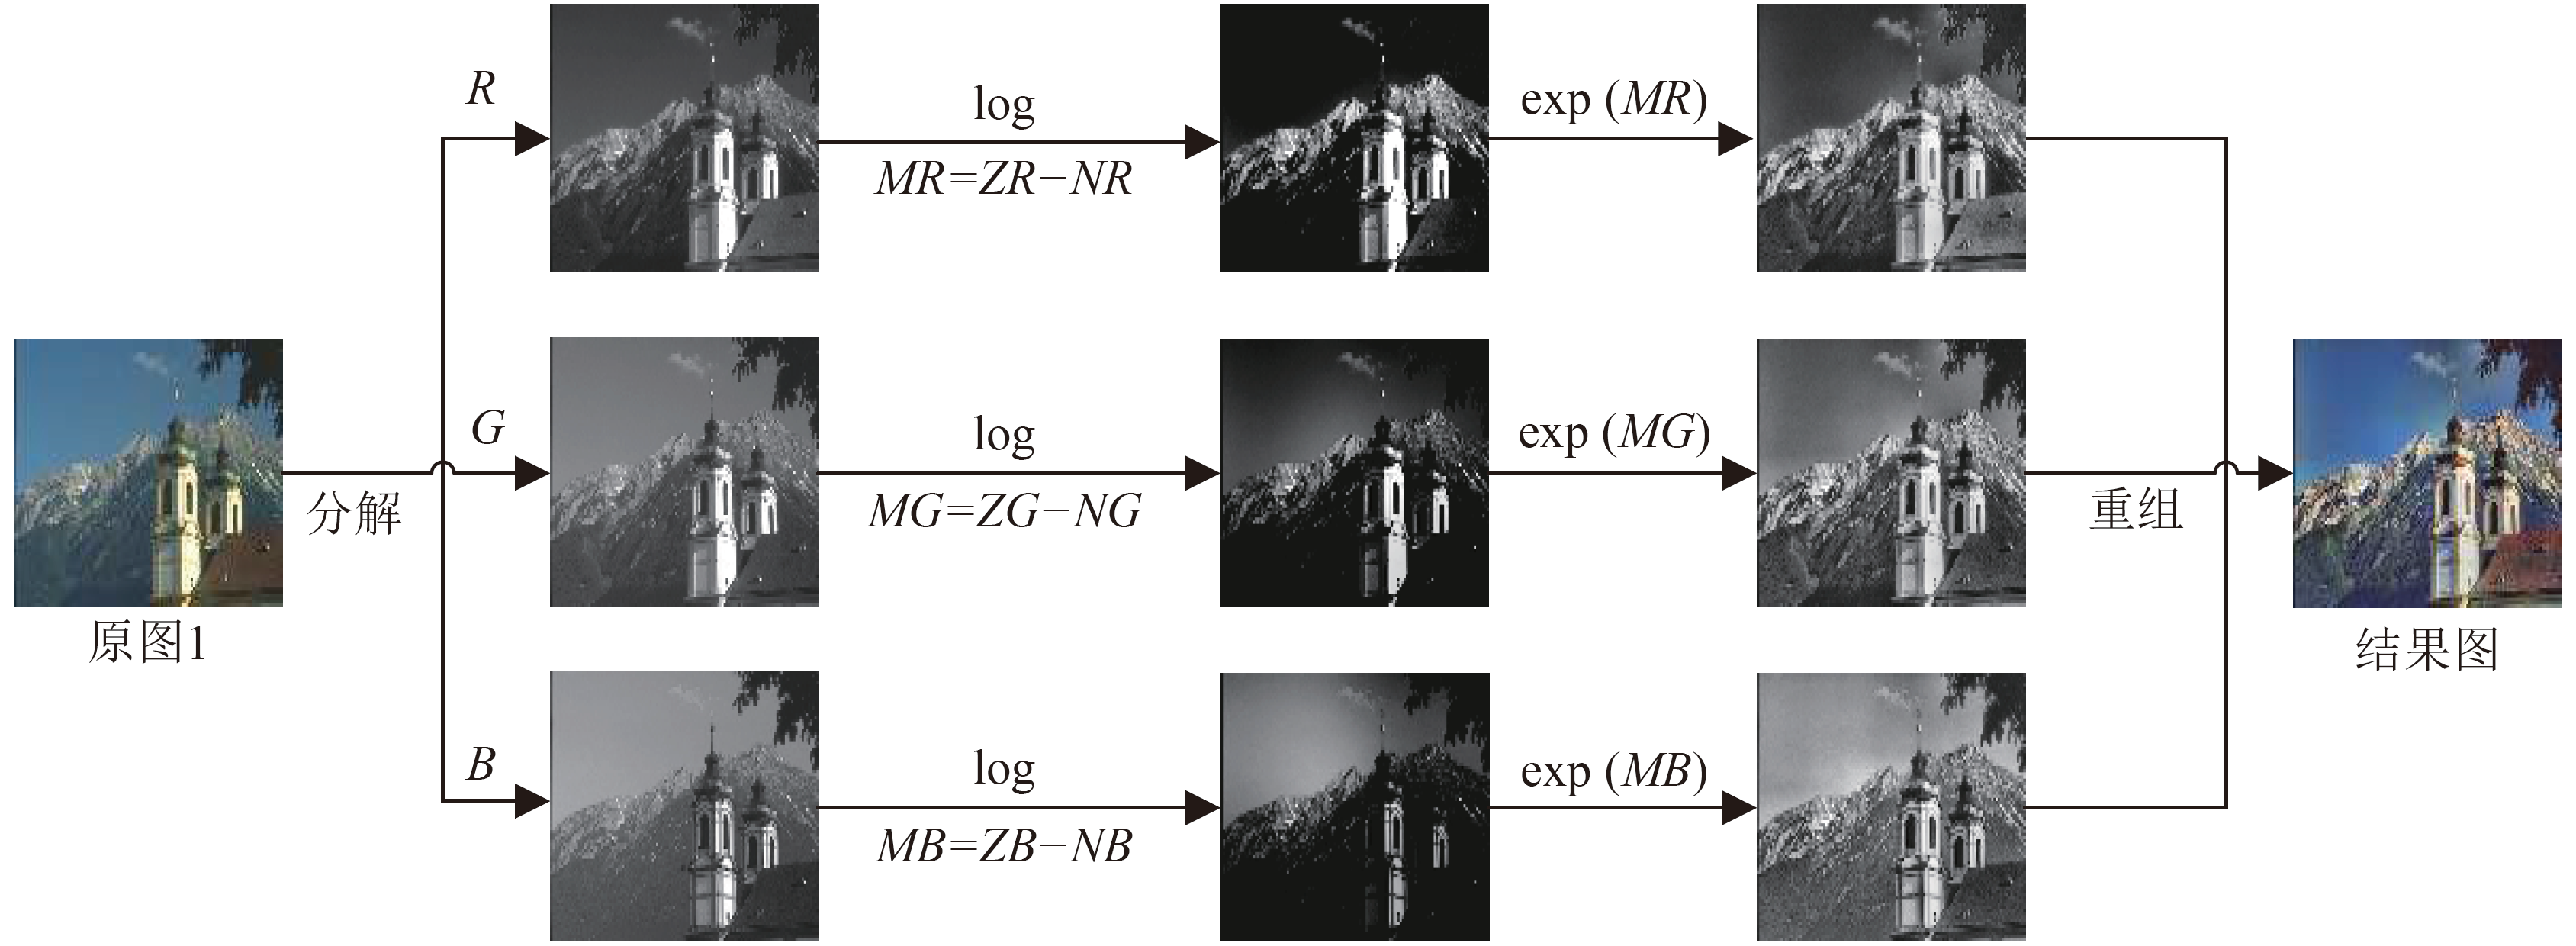
\includegraphics[width=0.5\columnwidth]{picture/LLIE/Retinex Model/Retinex Model}
			%\captionsetup{font=scriptsize}
			\caption{
				\label{fig: Retinex model} 
				\tiny Retinex 算法处理过程
			}
		\end{figure}
	\end{frame}
	
	\begin{frame}
		{\zihao{-5} \yahei \textbf{传统的弱光图像增强方法}}
		
		\begin{figure}[htbp] 
			\centering
			\setlength{\abovecaptionskip}{-0.03cm}
			\begin{minipage}{0.18\textwidth}
				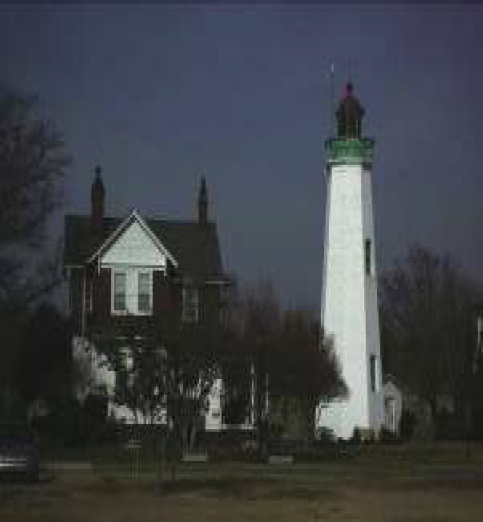
\includegraphics[width=\linewidth]{picture/LLIE/Retinex Model/input}
				\captionsetup{font=scriptsize}
				\caption*{\tiny input}
				\label{fig: Retinex Model_input}
			\end{minipage}
			\begin{minipage}{0.18\textwidth}
				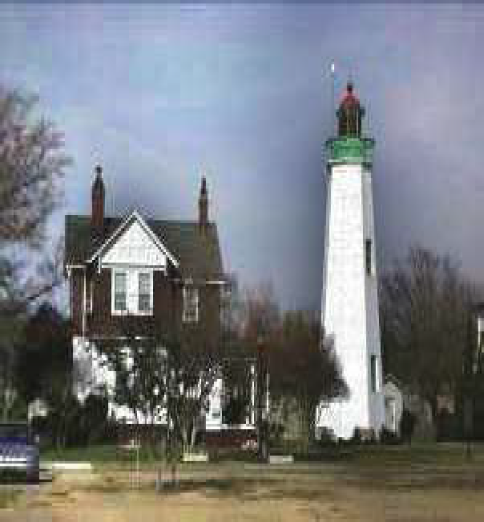
\includegraphics[width=\linewidth]{picture/LLIE/Retinex Model/Retinex}
				\captionsetup{font=scriptsize}
				\caption*{\tiny \textcolor{blue}{\citep{cooper2004analysis}}}
				\label{fig: Retinex Model_Retinex}
			\end{minipage}
			\begin{minipage}{0.18\textwidth}
				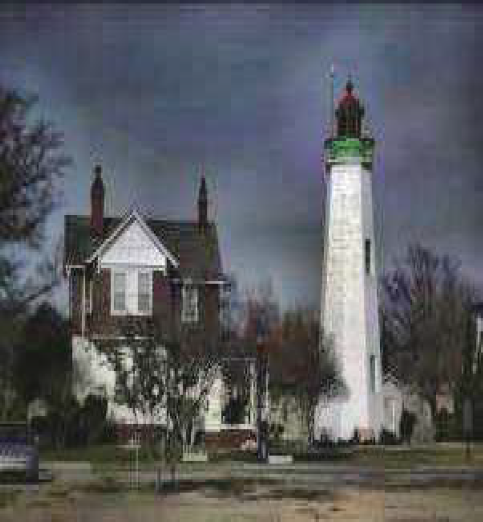
\includegraphics[width=\linewidth]{picture/LLIE/Retinex Model/SSR}
				\captionsetup{font=scriptsize}
				\caption*{\tiny SSR}
				\label{fig: Retinex Model_SSR}	
			\end{minipage}
			\begin{minipage}{0.18\textwidth}
				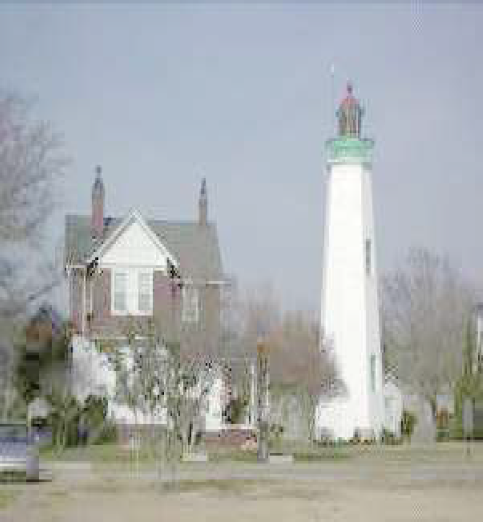
\includegraphics[width=\linewidth]{picture/LLIE/Retinex Model/MSR}
				\captionsetup{font=scriptsize}
				\caption*{\tiny MSR}
				\label{fig: Retinex Model_MSR}	
			\end{minipage}
			\begin{minipage}{0.18\textwidth}
				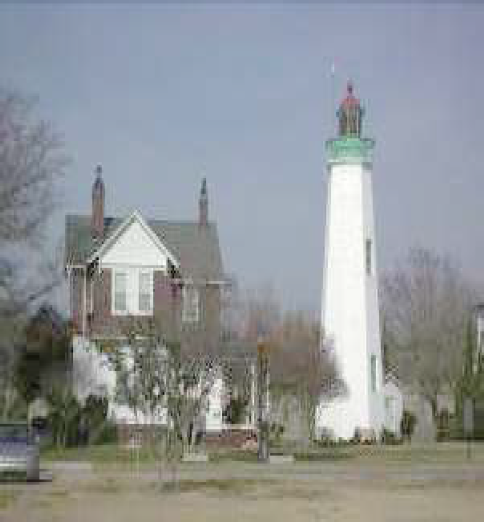
\includegraphics[width=\linewidth]{picture/LLIE/Retinex Model/MSRCR}
				\captionsetup{font=scriptsize}
				\caption*{\tiny MSRCR}
				\label{fig: Retinex Model_MSRCR}	
			\end{minipage}
			\captionsetup{font=scriptsize}
			\caption{
				\label{fig: Retinex Model}
				\tiny 传统 Retinex 算法实验结果。
			}
		\end{figure}
		
		{\zihao{-6} \yahei Retinex 模型在处理过程中往往忽视了噪声问题,这可能导致在反射图中产生大量噪声。反射图的计算本身是一个不稳定的问题,通常需要通过近似方法来估计。}
	\end{frame}
	
	\begin{frame}
		{\zihao{-5} \yahei \textbf{传统的弱光图像增强方法}}
		
		{\zihao{-6} \yahei 直方图均衡化通过对直方图的分布进行约束,改善图片的亮度分布。直方图描述了图像灰度级的分布情况,显示了图像的灰度范围和每个灰度级的出现频率。摄影师也常利用直方图判断整幅图像的明暗程度、对比度等图像特征,以便完成相应的后期处理。}
		
		\begin{figure}
			\centering			
			\begin{minipage}{.4\columnwidth}
				\begin{itemize}
					\item \zihao{-6} \yahei \textbf{直方图均衡化}
					
					\item[\checkmark]
					\zihao{-6} \yahei 快速有效,可逆操作				
					
					\item[\checkmark]
					\zihao{-6} \yahei 不加选择地处理数据,增加背景噪声的对比度.
				
					\item[\checkmark]
					\zihao{-6} \yahei 降低图像内容的对比度,导致视觉效果欠佳。
					
					\item[\checkmark]
					\zihao{-6} \yahei ......
					
				\end{itemize}
			\end{minipage}
			\begin{minipage}{.55\columnwidth}
				\setlength{\abovecaptionskip}{-0.05cm}
				\centering 
				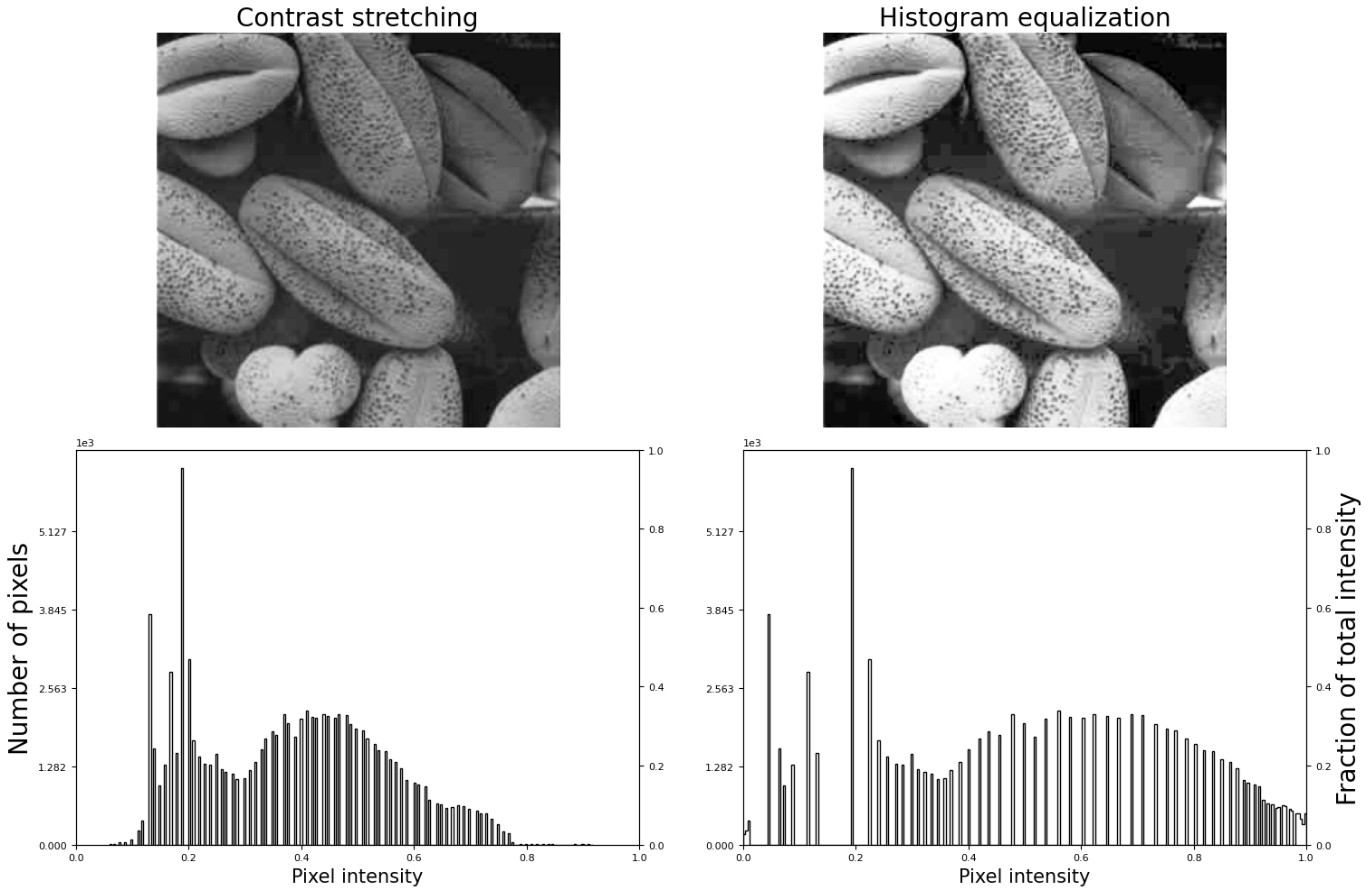
\includegraphics[width=\columnwidth]{picture/LLIE/HE/Histogram equalization}
				%\captionsetup{font=scriptsize}
				\caption{
					\label{fig: Histogram equalization} 
					\tiny 直方图均衡化示意图
				}
			\end{minipage}
		\end{figure}
		
	\end{frame}
	
	\subsubsection{基于深度学习的低照度图像增强方法}
	
	\begin{frame}
		{\zihao{-5} \yahei \textbf{基于深度学习的弱光图像增强方法}}
		
		{\zihao{-6} \yahei 从2017年LLNet\textcolor{blue}{\citep{lore2017llnet}}的出现,基于深度学习的低照度图像增强方法受到广泛关注,截至2023年已经出现了上百种基于深度学习的低照度图像增强方法,这充分反映了基于深度学习的方法具有更好的准确性、鲁棒性和更快的速度。}
		
		\vspace{0.1cm}
		
		{\zihao{-6} \yahei 基于深度学习的低照度图像增强算法,根据其学习和训练方式又分为四类,分别为有监督学习、无监督学习、半监督学习和零采样(Zero-shot)学习方法\textcolor{blue}{\citep{tang2023low}}。}
		
		\vspace{0.1cm}
		
		\begin{figure}
			\centering
			\setlength{\abovecaptionskip}{-0.05cm}			
			\begin{minipage}{.4\columnwidth}
				\setlength{\abovecaptionskip}{-0.05cm}
				\centering 
				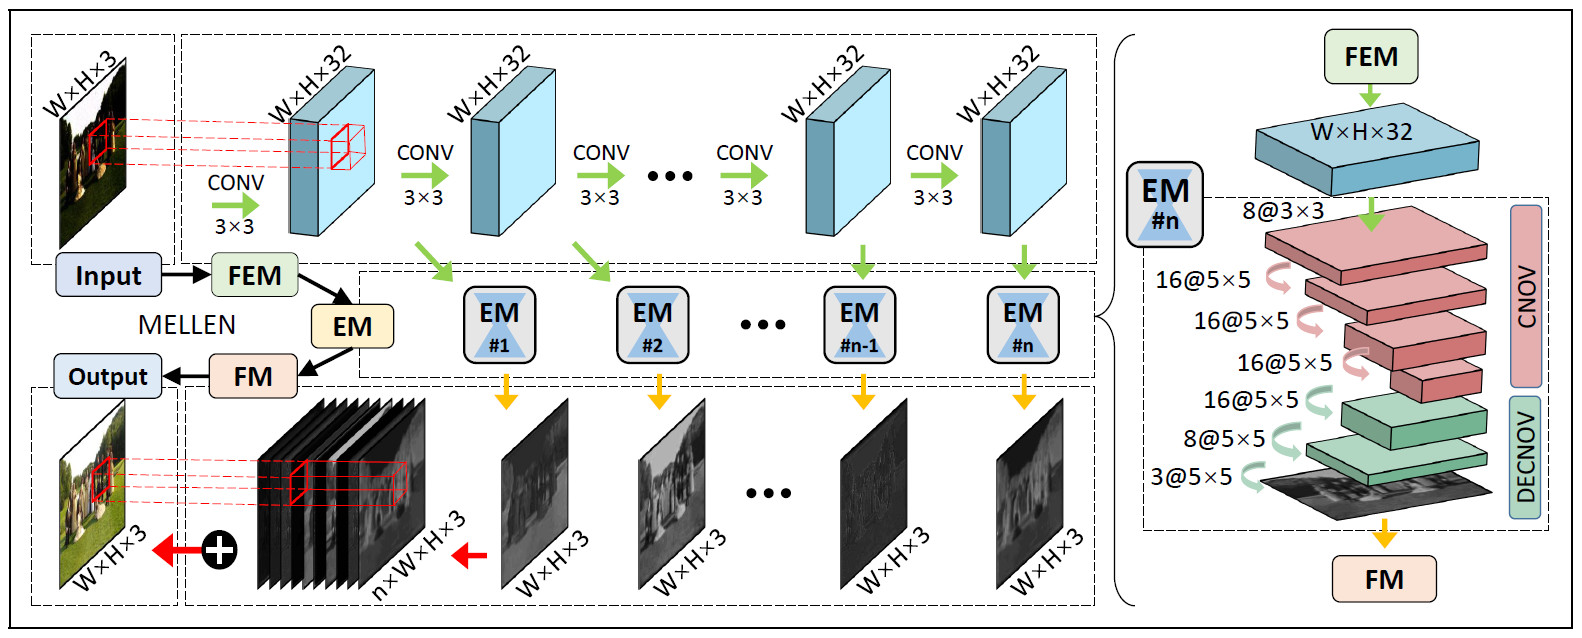
\includegraphics[width=\columnwidth]{picture/LLIE/MBLLEN/MBLLEN Architecture}
				%\captionsetup{font=scriptsize}
				\caption{
					\label{fig: MBLLEN} 
					\tiny MBLLEN 结构示意图
				}
			\end{minipage}
			\begin{minipage}{.4\columnwidth}
				\setlength{\abovecaptionskip}{-0.05cm}
				\centering 
				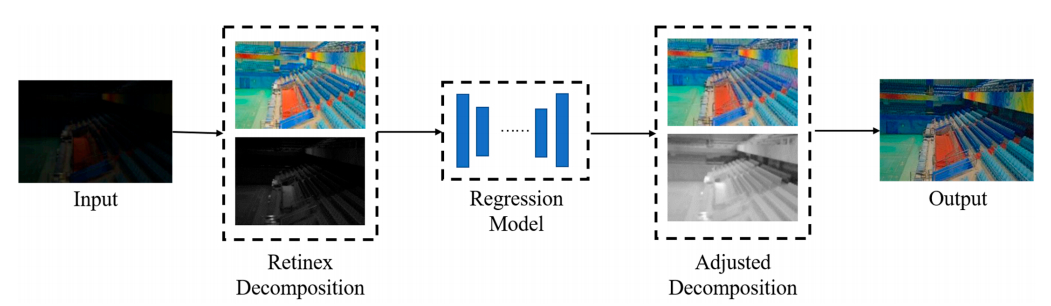
\includegraphics[width=\columnwidth]{picture/LLIE/RetinexNet/RetinexNet}
				%\captionsetup{font=scriptsize}
				\caption{
					\label{fig: RetinexNet} 
					\tiny RetinexNet 结构示意图
				}
			\end{minipage}
			\captionsetup{font=scriptsize}
			\caption{
				\label{fig: Supervised Learning}
				\tiny 经典有监督学习架构
			}
		\end{figure}
		
	\end{frame}
	
	\begin{frame}
	{\zihao{-5} \yahei \textbf{基于深度学习的弱光图像增强方法}}
	
	{\zihao{-6} \yahei 尽管有监督学习方法在图像增强中取得了一定的成效,但它面临着两大主要限制。首先,可用于训练的成对图像数据集是有限的。其次,在这样的成对数据集上训练的模型容易出现过拟合的问题。为了克服这些挑战,研究者们转向了无监督学习方法。}
	
	{\zihao{-6} \yahei Jiang等人\textcolor{blue}{\citep{jiang2021enlightengan}}开创性地提出了一种名为 \textbf{EnlightenGAN} 的无监督学习方法。}
	
	\begin{figure}
		\centering
		\setlength{\abovecaptionskip}{-0.05cm}
		\begin{minipage}{.6\columnwidth}
			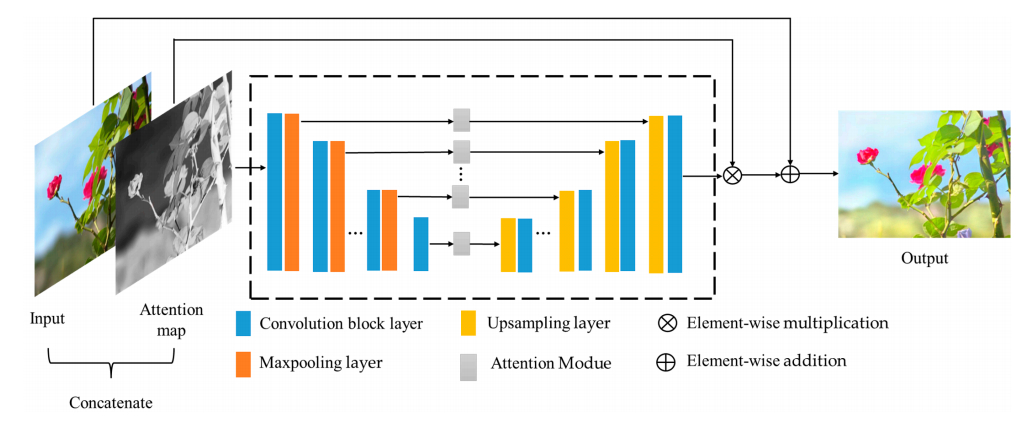
\includegraphics[width=\columnwidth]{picture/LLIE/EnlightenGAN/EnlightenGAN}
			\caption{
				\label{fig: EnlightenGAN Architecture} 
				\tiny EnlightenGAN 结构图
			}
		\end{minipage}
	\end{figure}
	
	{\zihao{-6} \yahei EnlightenGAN的主要创新在于两个方面:一是其全局-局部判别器结构,用于处理输入图像中的空间光照变化;二是结合自特征保留损失和自正则化注意力机制,确保增强后图像的内容特征保持不变。}
	
	\end{frame}
	
	\begin{frame}
		{\zihao{-5} \yahei \textbf{基于深度学习的弱光图像增强方法}}
		
		{\zihao{-6} \yahei 近年来,半监督学习作为一种新兴的学习方法,结合了监督学习的精确性和非监督学习的广泛适用性。这种学习方法既利用了有标签的数据,也依赖于无标签的数据。Yang等人\textcolor{blue}{\citep{qiao2021deep}}提出了一种名为 \textbf{DRBN} 的半监督低照度图像增强方法,该方法基于频带表示。}
		
		\begin{figure}
			\centering
			\setlength{\abovecaptionskip}{-0.05cm}
			\begin{minipage}{.7\columnwidth}
				\centering 
				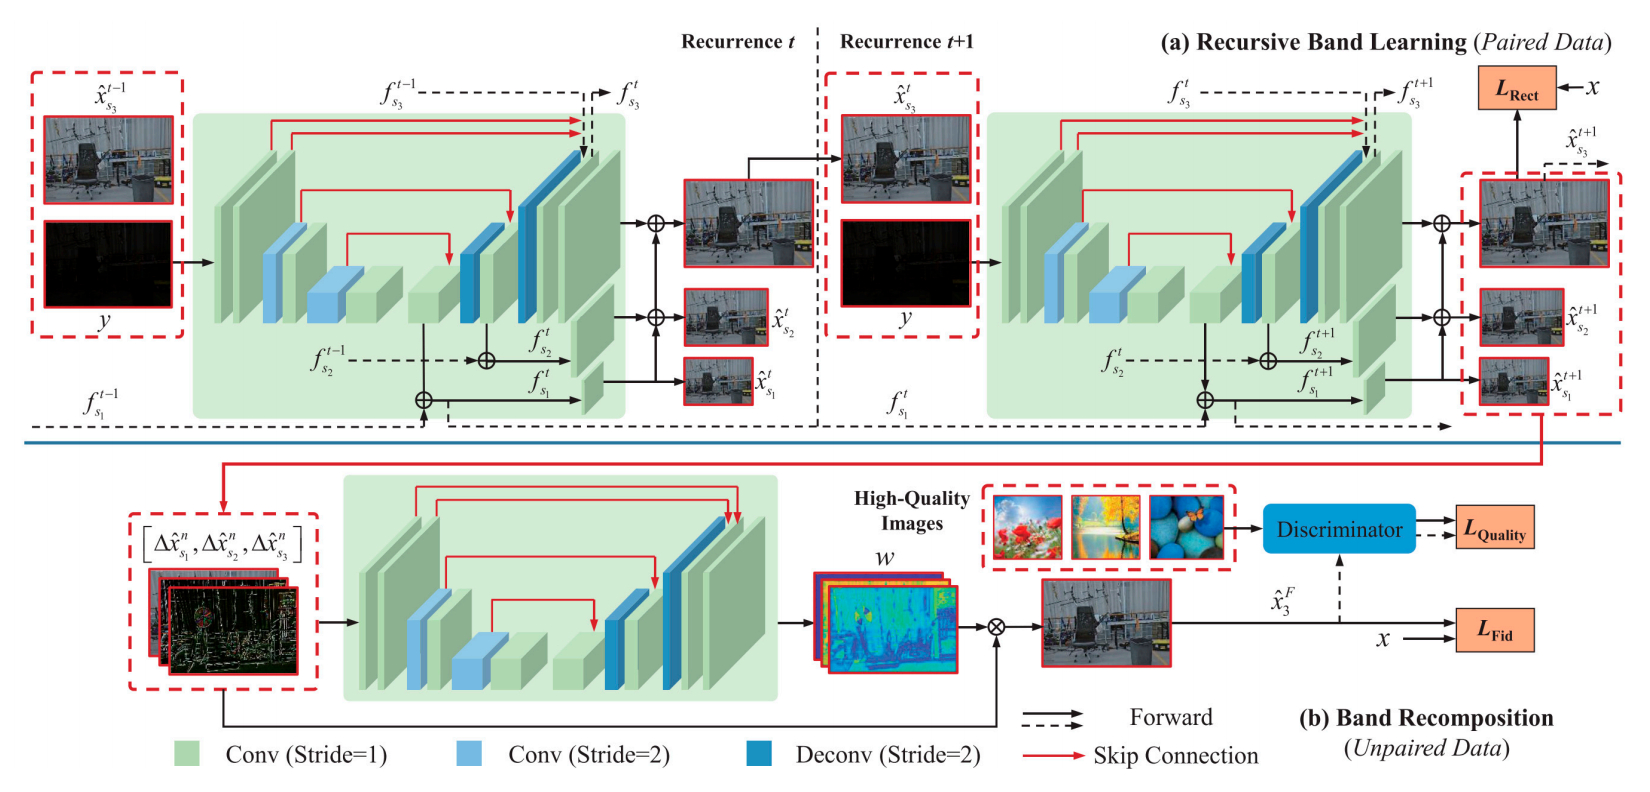
\includegraphics[width=\columnwidth]{picture/LLIE/DRBN/DRBN}
				\caption{
					\tiny DRBN 结构图
				}
			\end{minipage}
		\end{figure}
		
	\end{frame}
	
	\begin{frame}
		{\zihao{-5} \yahei \textbf{基于深度学习的弱光图像增强方法}}
		
		{\zihao{-6} \yahei Zero-shot 学习的一个显著优点是它无需依赖预先训练的数据集。这种方法允许直接将待处理的低光照图像作为输入,而无需经过预先的训练阶段。Zhu等人\textcolor{blue}{\citep{zhu2020zero}}提出了一种创新的三分支全卷积神经网络,名为\textbf{RRDNet}。}
		
		\begin{figure}
			\centering
			\setlength{\abovecaptionskip}{-0.05cm}
			\begin{minipage}{.6\columnwidth}
				\centering 
				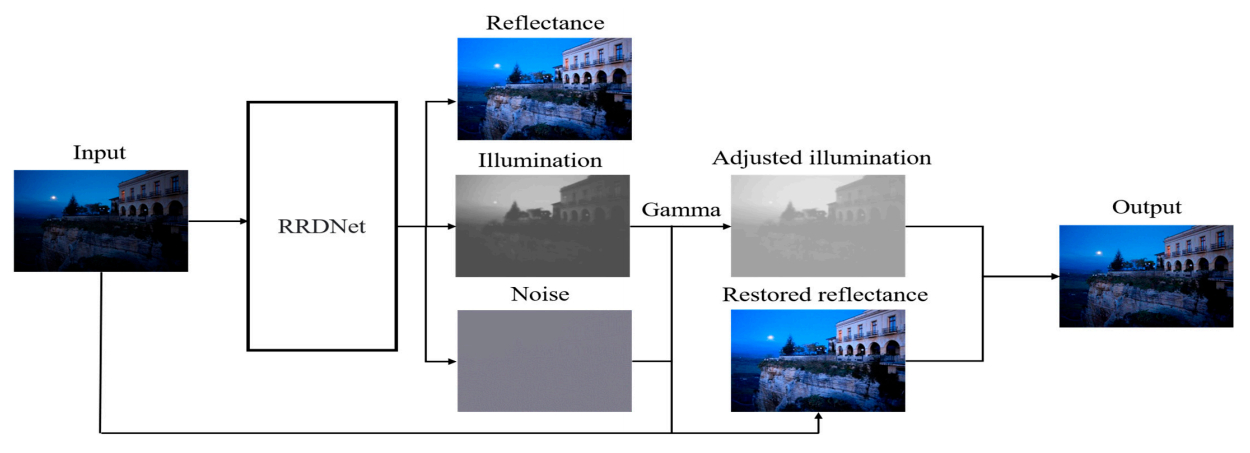
\includegraphics[width=\columnwidth]{picture/LLIE/RRDNet/RRDNet}
				\caption{
					\tiny RRDNet 结构图
				}
			\end{minipage}
		\end{figure}
		
		{\zihao{-6} \yahei 该网络将输入图像拆分为三个组成部分:光照、反射和噪声。通过特殊设计的迭代损失函数,网络能够对噪声进行精确估计并有效恢复光照部分,实现清晰的噪声预测,进而成功去除图像中的噪声。}
		
	\end{frame}
	
	\begin{frame}
		{\zihao{-5} \yahei \textbf{基于Transformer的弱光图像增强方法}}
		
		{\zihao{-6} \yahei Transformer架构\textcolor{blue}{\cite{vaswani2017attention}}在图像处理领域的应用以来\textcolor{blue}{\cite{dosovitskiy2020image}},其在捕获全局特征方面的能力引起了行业的广泛关注。}
		
		\begin{figure}
			\centering
			\setlength{\abovecaptionskip}{-0.05cm}
			\begin{minipage}{.6\columnwidth}
				\centering
				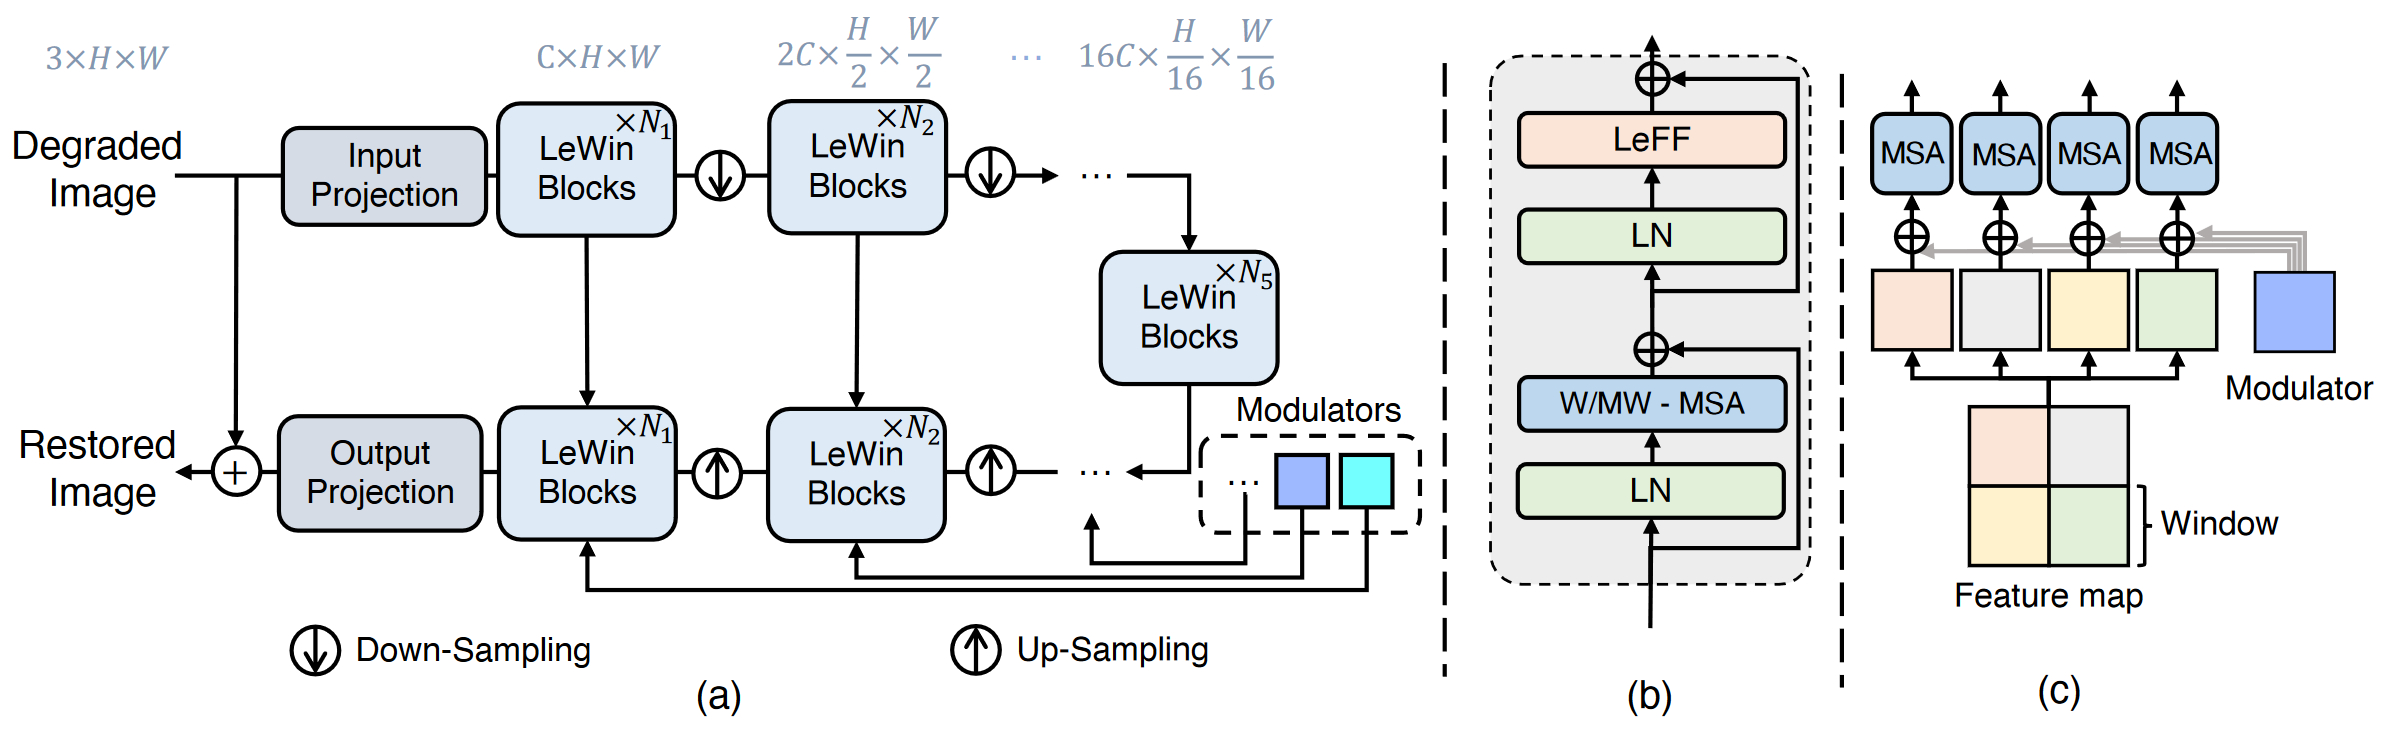
\includegraphics[width=\columnwidth]{picture/LLIE/Uformer/Uformer}
				%\captionsetup{font=scriptsize}
				\caption{
					\label{fig: Uformer} 
					\tiny Uformer 的结构。
				}
			\end{minipage}
		\end{figure}
		
		{\zihao{-6} \yahei 为了缓解计算负担,部分研究工作尝试采用局部窗口策略来限制自注意力机制的计算范围,并借鉴 U-Net 架构,引入跳过连接机制以增强特征传递\textcolor{blue}{\cite{wang2021uformer}}。}
		
		%尽管这种方法在降低计算成本方面取得了一定成效,但它可能会削弱Transformer架构在捕获图像中长距离特征的能力,进而影响其在图像复原任务中的整体性能。
		
		%为了克服这一限制,提出的解决方案\cite{chen2023cross}主要集中在窗口间的交互和与卷积神经网络(CNN)模块的耦合上。这种方法旨在将CNN的平移不变性和局部性归纳偏差融入Transformer架构中,从而实现两者优势的互补。我们将这类解决方案称为CNN与Transformer的串联策略。
	\end{frame}
	
	\subsection{研究目的}
	
	\begin{frame}
		{\zihao{-4} \yahei \textbf{研究目的}}
		
		\begin{figure}
		\begin{minipage}{.4\columnwidth}
			\begin{itemize}
				\item \zihao{-5} \yahei \textbf{现有方法存在的局限性}
				
				\item[\XSolidBrush]
				\zihao{6} \yahei 在提高亮度的同时,无法很好的消除产生的噪声。
				
				\item[\XSolidBrush]
				\zihao{6} \yahei 一些方法无法很好的避免颜色失真现象。
				
				\item[\XSolidBrush]
				\zihao{6} \yahei 现有的方法往往不具备鲁棒性。
				% 一些现有的方法可以有效地解决一个问题,但往往会忽略了其他问题。不同的方法在不同的数据集上往往具有不同的优势,即在不同的评估标准下有不同的优势。
				\item[\XSolidBrush]
				\zihao{6} \yahei 无法在极暗或极亮的区域很好地恢复图像边缘细节\textcolor{blue}{\citep{xu2023low}}。
				
				\vspace{0.2cm}
				
				{\zihao{-6} \yahei 在暗区域中加入敏感边缘先验可以降低优化外观重构时的不适定程度\textcolor{blue}{\citep{xu2023low}}。一些框架\textcolor{blue}{\citep{rana2021edge}}\textcolor{blue}{\citep{zhu2020eemefn}}使用基于编码器-解码器的网络和回归损失执行结构建模。然而,由于能见度和噪声严重不足导致的暗区不确定性,相应的结构建模结果并不令人满意。}
			\end{itemize}
		\end{minipage}
		\begin{minipage}{.58\columnwidth}
			\setlength{\abovecaptionskip}{-0.05cm}
			\centering 
			\begin{minipage}{0.3\textwidth}
				\centering
				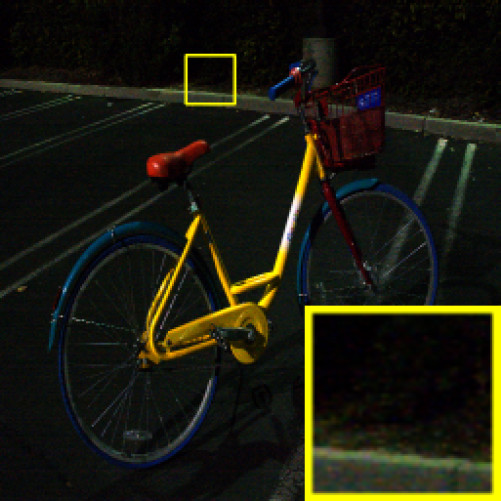
\includegraphics[width=.8\linewidth]{picture/LLIE/Structure Modeling and Guidance/Input}
				\caption*{\tiny (a) Input}
			\end{minipage}
			\begin{minipage}{.3\textwidth}
				\centering
				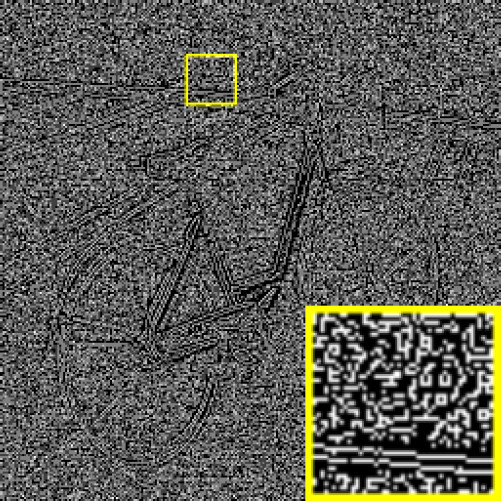
\includegraphics[width=.8\linewidth]{picture/LLIE/Structure Modeling and Guidance/Structure of (a)}
				\caption*{\tiny (b) Structure of input}
			\end{minipage}
			\begin{minipage}{.3\textwidth}
				\centering
				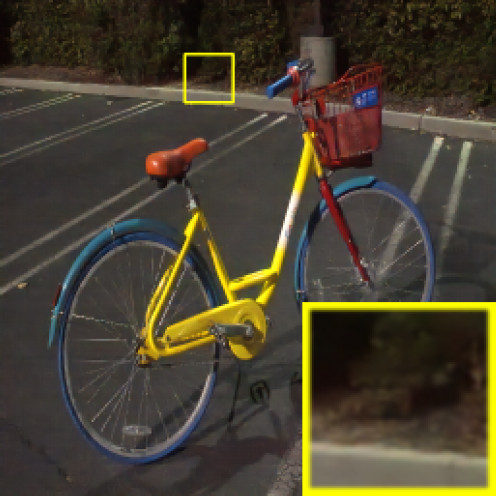
\includegraphics[width=.8\linewidth]{picture/LLIE/Structure Modeling and Guidance/SNR (CVPR 2022)}
				\caption*{\tiny (c) SNR (CVPR 2022)}
			\end{minipage}
			\begin{minipage}{.3\textwidth}
				\centering
				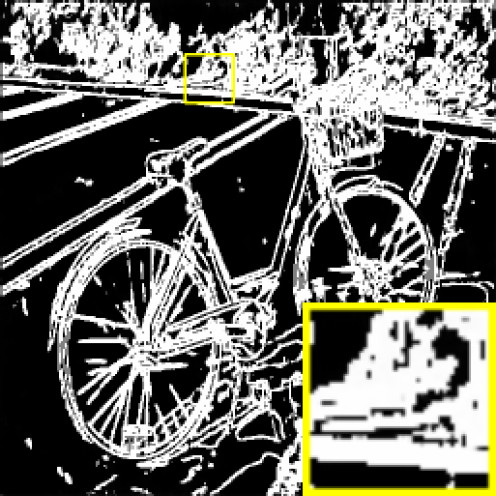
\includegraphics[width=.8\linewidth]{picture/LLIE/Structure Modeling and Guidance/Structure Modeling}
				\caption*{\tiny (d) Structure Modeling}
			\end{minipage}
			\begin{minipage}{.3\textwidth}
				\centering
				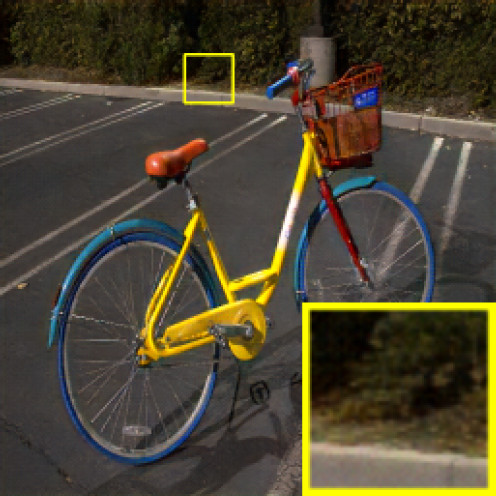
\includegraphics[width=.8\linewidth]{picture/LLIE/Structure Modeling and Guidance/Ours}
				\caption*{\tiny (e) Ours}
			\end{minipage}
			\begin{minipage}{.3\textwidth}
				\centering
				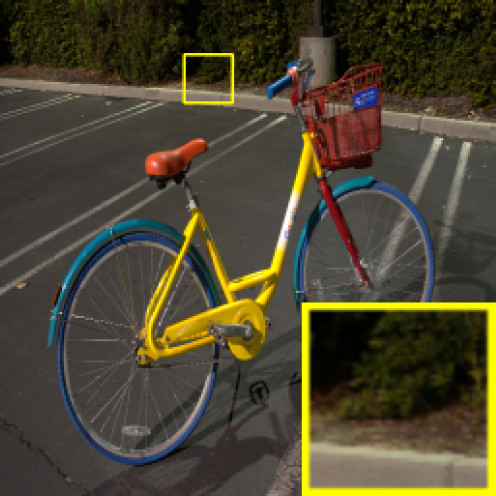
\includegraphics[width=.8\linewidth]{picture/LLIE/Structure Modeling and Guidance/Ground Truth}
				\caption*{\tiny (f) Ground Truth}
			\end{minipage}
			\caption{
				\tiny SID-sRGB\textcolor{blue}{\citep{chen2018learning}}中一张弱光图片, 通过SOTA方法 (c) 和  \textcolor{blue}{\citep{xu2023low}} 提出的方法 (e)增强。作者的方法可以从输入的图像中合成结构图(d),使细节更清晰,对比度更清晰,颜色更鲜艳。虽然(c)的 PSNR 为 28.17,但其 SSIM 低为 0.75。作者的方法在dB和SSIM的得分都很高,分别为28.60 dB 和 0.80。
			}
		\end{minipage}
		\end{figure}
		
	\end{frame}
	
	\begin{frame}
		\begin{figure}
			\centering
			\setlength{\abovecaptionskip}{-0.05cm}
			\begin{minipage}{0.45\columnwidth}
				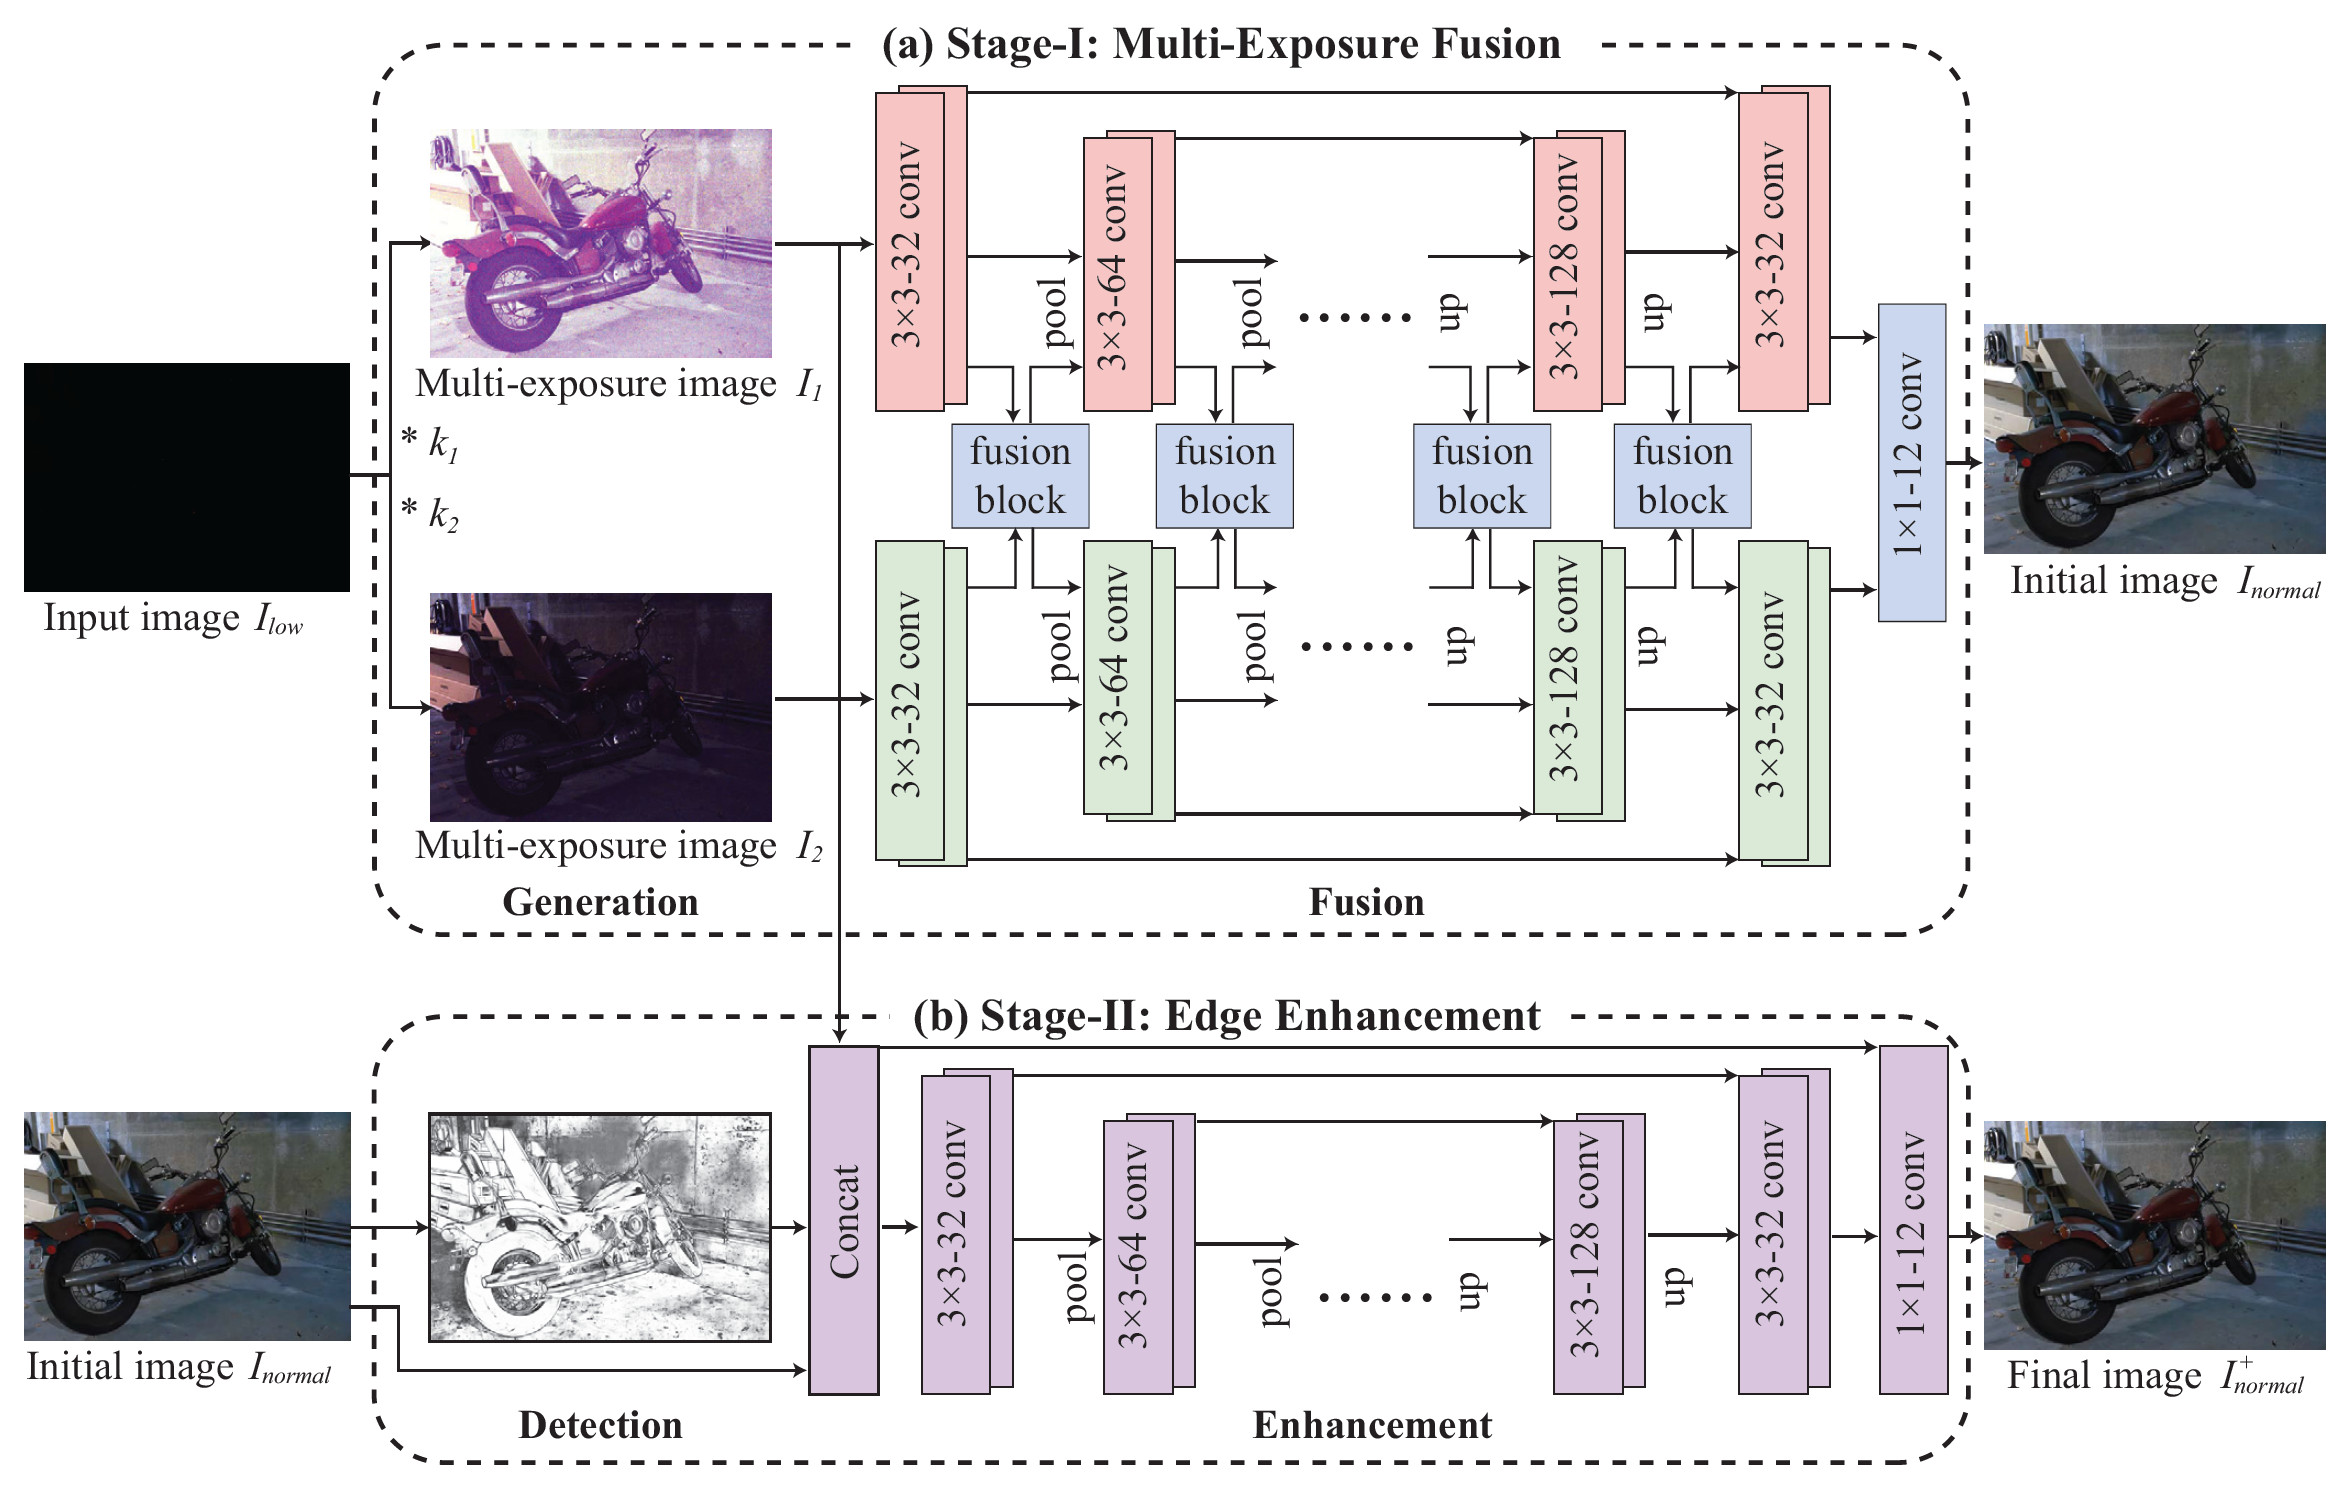
\includegraphics[width=\linewidth]{picture/LLIE/EEMEFN/EEMEFN framework}
				\caption*{\tiny
					(a) 该 LLIE 结构源自\cite{zhu2020eemefn},如其 Multi-Exposure Fusion 部分采用多曝光融合结构,与由 Initial image 生成的边缘图进行 Concat, 后续通过一个 U-Net 网络进一步恢复图像。}
			\end{minipage}
			\begin{minipage}{0.45\columnwidth}
				\setlength{\abovecaptionskip}{0.29cm}
				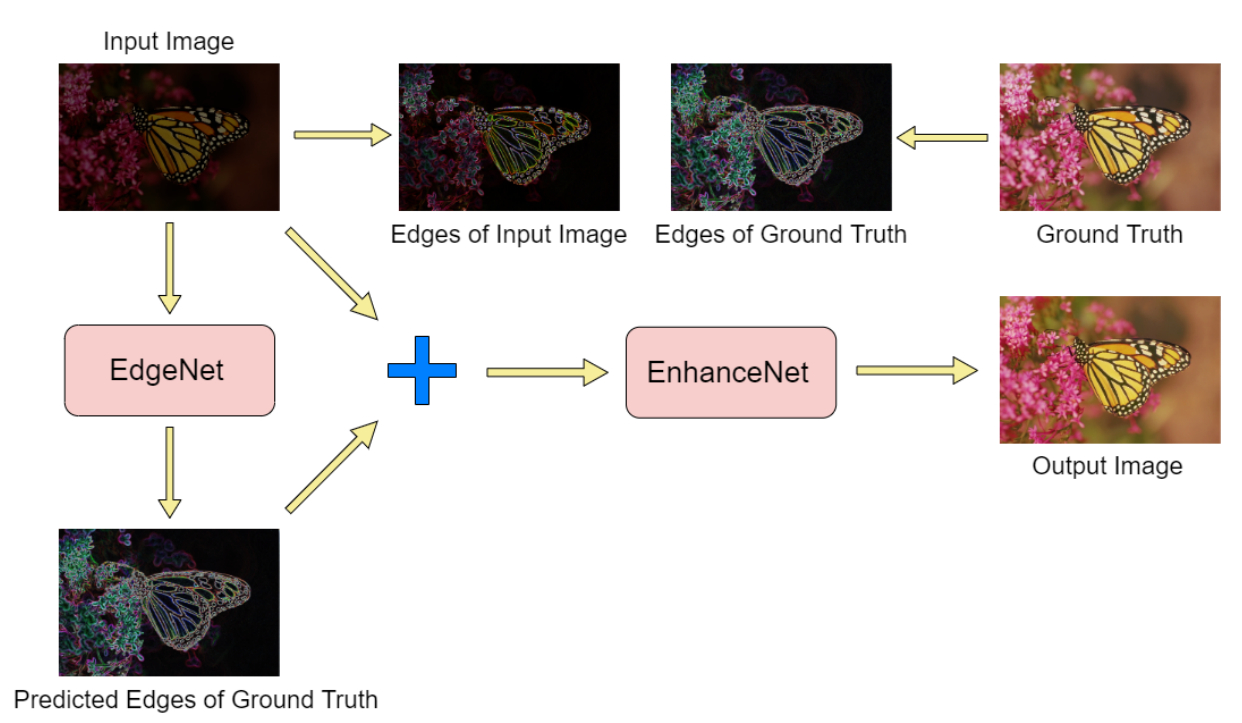
\includegraphics[width=\linewidth]{picture/LLIE/EdgeNet/Archtecture workflow}
				\caption*{\tiny
					(b) 该 LLIE 结构源自\cite{rana2021edge}使用 EdgeNet 首先从低光图像中过滤边缘,EnhanceNet 反复使用上采样和下采样块的组合,从局部到全局逐渐提取特征,并消除伪影和噪声。}
			\end{minipage}
			\caption{\tiny 边缘图像指导弱光图像增强的传统架构。}
		\end{figure}
		
		\vspace{-0.5cm}
		
		\begin{minipage}{.9\textwidth}
			\textbf{\tiny 具有的特点}
			\begin{itemize} \tiny
				\item [\checkmark] 其恢复结果的质量会受到\textcolor{red}{增强网络的设计}和\textcolor{red}{初步恢复图像与边缘结构图生成质量}的影响。
				
				\item [\checkmark] 边缘图的准确性会极大影响最终的恢复结果,直接从弱光图像中获取边缘图具有一定的挑战性。
				
				\item [\checkmark] 边缘图与初步恢复图像之间多采用\textcolor{red}{串联方式}输入卷积以获得最终增强结果。
			\end{itemize}
		\end{minipage}
		
	\end{frame}	
	
	\begin{frame}
		\begin{figure}[htbp]
			\begin{center}
				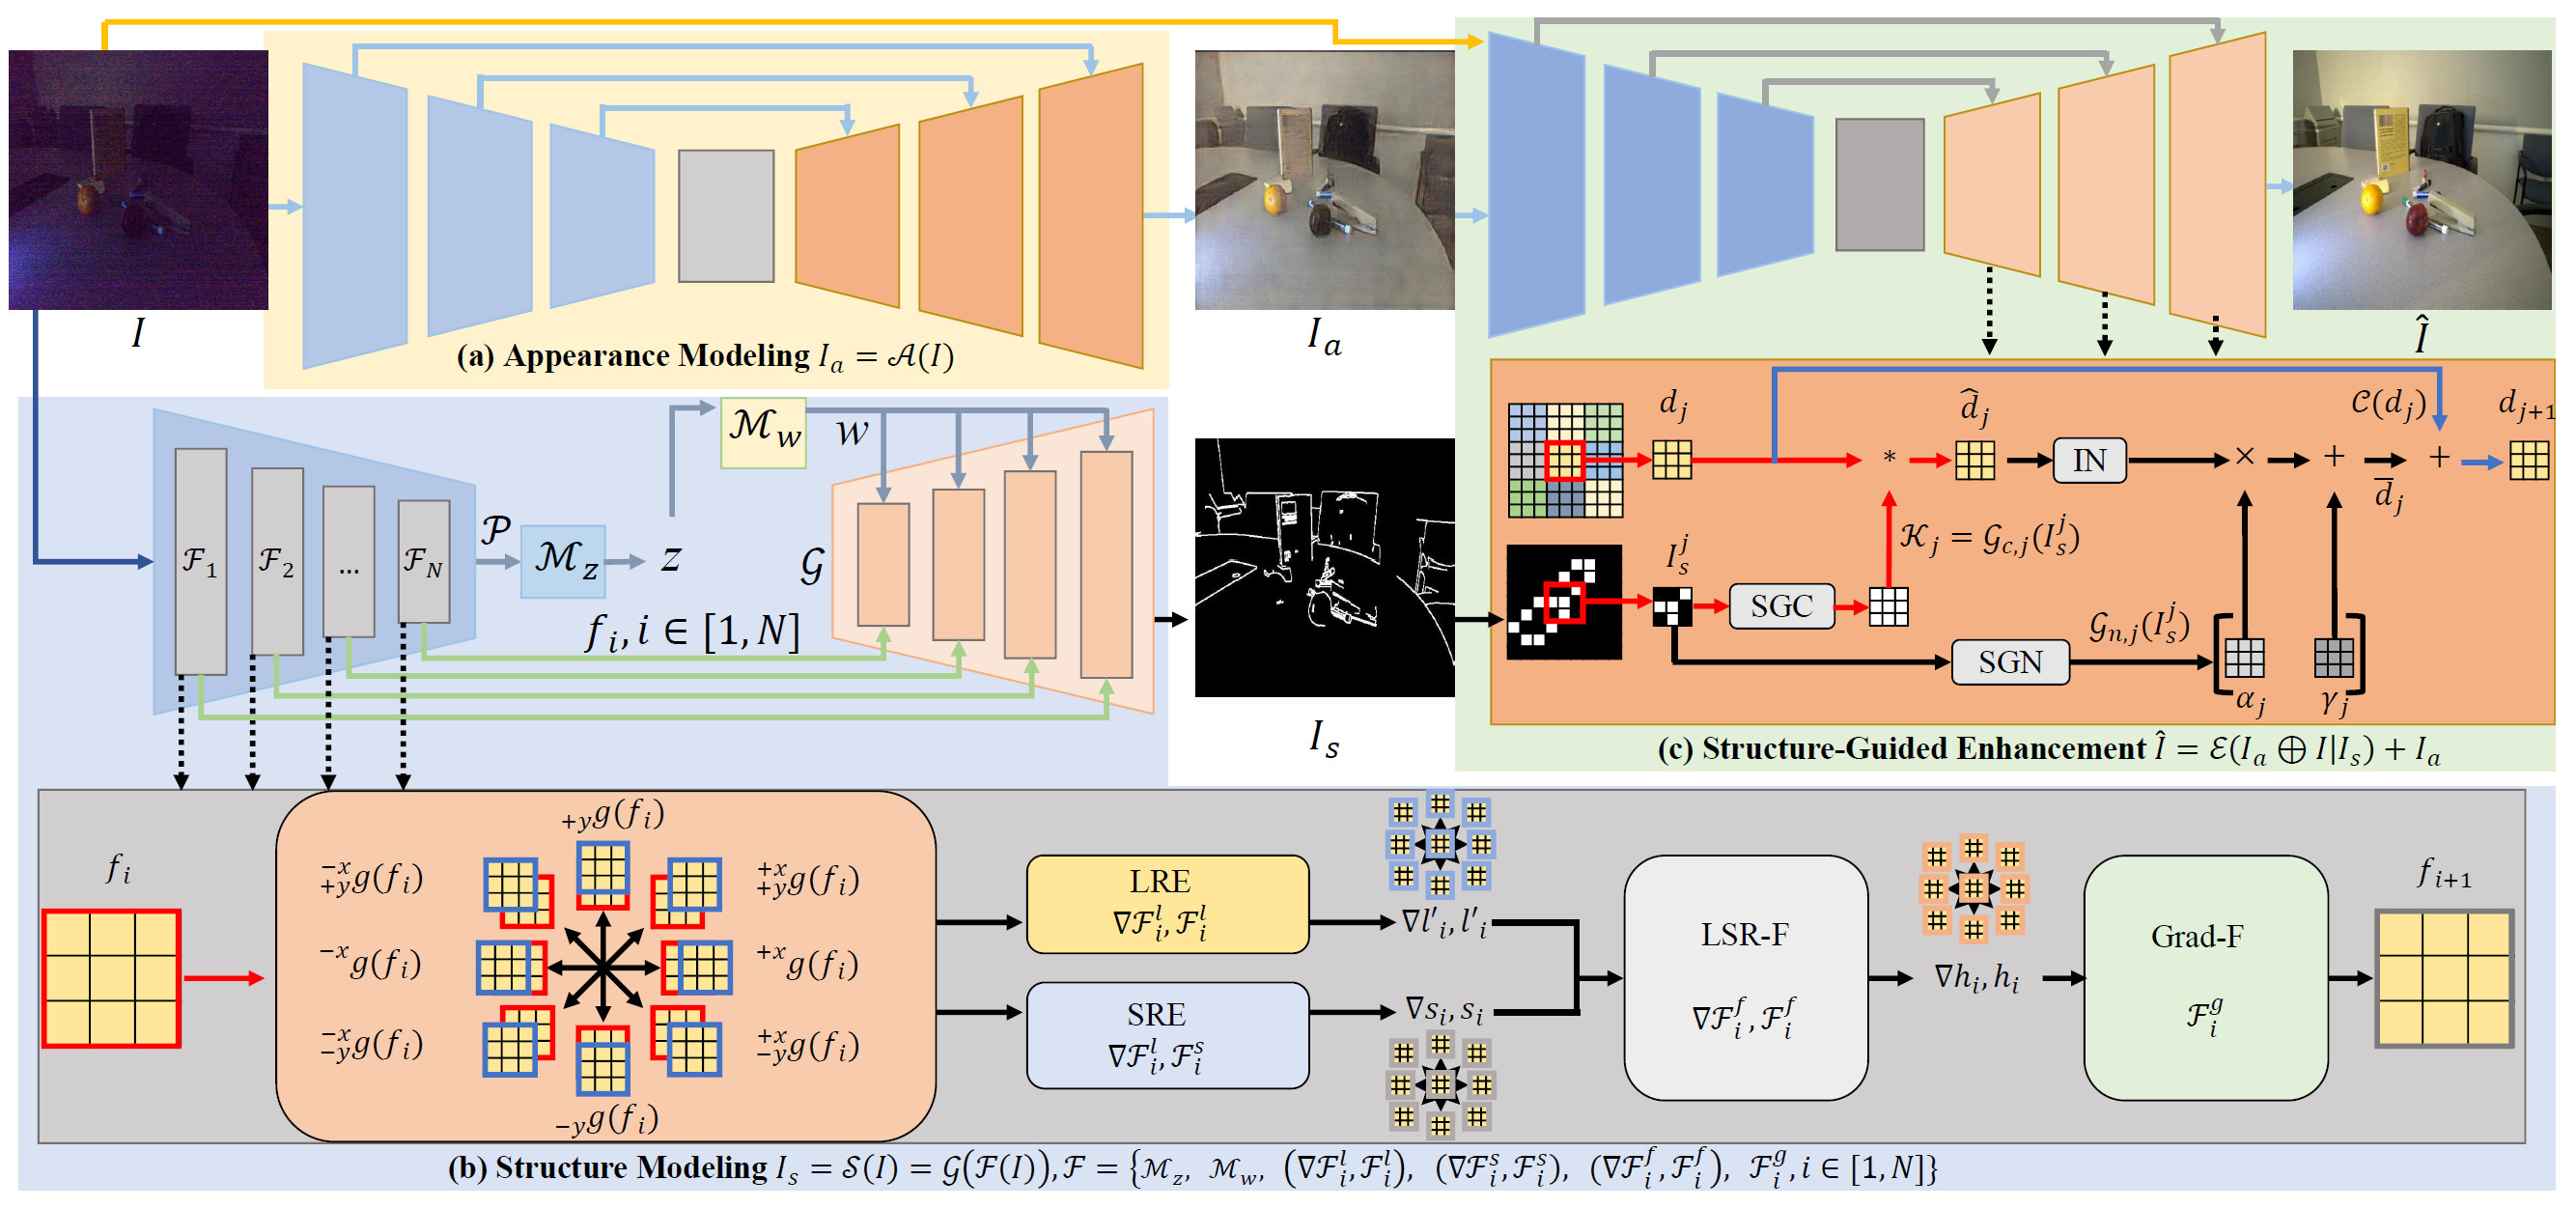
\includegraphics[width=0.8\textwidth]{picture/LLIE/Structure Modeling and Guidance/Overview}
				\caption{
					\tiny 该 LLIE 结构源自\textcolor{blue}{\cite{xu2023low}},其提出一种基于 GAN Loss 的模型去对结构信息建模,通过获得的结构信息指导增强。
				}
			\end{center}
		\end{figure}
		
		\vspace{-0.5cm}
		
		\begin{minipage}{.6\textwidth}
			\textbf{\tiny 具有的特点}
			\begin{itemize} \tiny
				\item [\checkmark] 传统架构无法很好的利用边缘信息语义指导恢复弱光图像。
				
				\item [\checkmark] 低光照中的图片很难提取到好的结构信息。
				
				\item [\checkmark] StyleGAN从弱光图像中提取出接近 GT 边缘图。
			\end{itemize}
		\end{minipage}
		\begin{minipage}{.3\textwidth}
			\textbf{\tiny 可以改进的点}
			\begin{itemize}\tiny
			\item [-] 未给出边缘网络模型的实验结果。
			% 论文指出低光数据集图片较少,所以结构信息提取模块的训练会受限,因此作者引入其他结构信息提取的数据集做额外训练可以进一步提升performance
			
			\item [-] 语义图和深度图可以作为引导信息。
			% 作者提出除了边缘结构图作为引导信息,也可以使用其他特征,比如语义图( Ours with SEG.)和深度图( Ours with Dep.),总体表现没有边缘图好,但是也比一些现有的增强方法好。
			
			\item [-] 可以使用不同的引导网络。
			% 作者没有说 Appearance Modeling 的结果去提取边缘会达到什么效果?
			
			% 此外作者做消融实验的过程中,使用一个 SOTA 边缘提取网络代替论文中的structural modeling 模块(但是感觉在低光照下很难提取到有效的边缘,合理点的话需要先对输入亮度增强一下)
			\end{itemize}
		\end{minipage}
	\end{frame}
	
	\begin{frame}
		{\zihao{-4} \yahei \textbf{本研究的研究目标}}
		
		\begin{itemize}\zihao{5}
			\item [-]
			边缘网络的开发
			%设计并构建一个创新的边缘网络,其核心功能是从低光照图像中直接提取边缘结构图。该网络生成的结构图应与地面真实(GT)生成的边缘结构图具有高度的相似性,从而确保准确性和可靠性。
			
			\vspace{-0.05cm}
			
			\item [-]
			初步恢复图像的生成模型
			%开发一个用于生成初步恢复图像的低光照图像增强模型。该模型应专注于从弱光条件下的图像中恢复清晰度和细节,以提高整体图像质量。
	
			\vspace{-0.05cm}
			
			\item [-]
			边缘语义信息的增强网络模型
			%在现有的直接串联方法基础上,进行创新性改进,构建一种更有效利用边缘语义信息的增强网络模型。目的在于通过这种改进,进一步提升图像增强过程中边缘结构的利用效率和效果。
		\end{itemize}
		
	\end{frame}
	
	\begin{frame}
		Conformer: Local Features Coupling Global presentations for Visual Recognition\textcolor{blue}{\citep{peng2021conformer}}
		\begin{itemize}
			\item \textbf{Background}
			\item[\checkmark]
			Transformer is introduced into the visual task. 
			% Transformer 被引入视觉任务
			
			\item[\checkmark]
			Vision Transformer reflect the complex spatial transformations and long-distance feature dependence.
			% 由于自注意力机制和多层感知器 MLP 结构,Vision Transformer反映了复杂的空间变换和远距离特征依赖,它们构成了全局表示。
			
			\item[\checkmark]
			Local feature details are ignored.
			% Vision Transformer 反映了复杂的空间变换和远距离特征以来,他们构成了全局表示。
		\end{itemize}
		
		\begin{figure}[htbp]
			\begin{center}
				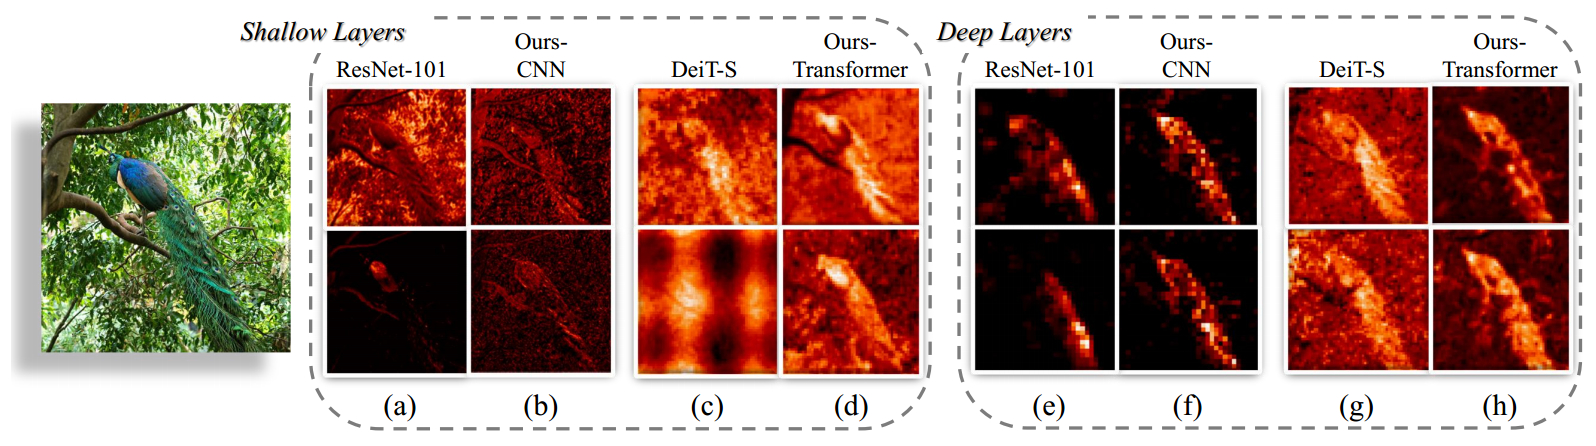
\includegraphics[width=0.8\textwidth]{picture/LLIE/Conformer/Comparison of feature maps of CNN (ResNet-101)}
			\end{center}
		\end{figure}
		
		% CNN (ResNet-101)、Visual Transformer (DeiT-S)和所提出的 Conformer 的特征图比较。变压器中的贴片嵌入被重塑为特征映射,以实现可视化。CNN 激活了判别性的局部区域(例如: 孔雀的头部(a)和尾部(e)), Conformer 的 CNN 分支利用了来自视觉变压器的全局线索,从而激活了完整的对象(例如: 孔雀的整个范围(b)和(f))。与 CNN 相比,视觉变压器的局部特征细节变差(例如: (c), (g))。Conformer的 Transformer 分支保留了 CNN 的局部特征细节,同时压制了背景(例如: (d)和(h)中的孔雀轮廓比(c)和(g)中的孔雀轮廓更完整)。(以彩色观看效果最佳)
	\end{frame}
	
	\begin{frame}

		\begin{figure}
			\centering
			\begin{minipage}{.4\textwidth}
				\centering
				\small
				\begin{itemize}
					\item \textbf{Contribution}
					
					\item[\checkmark]
					A Dual Network Structure
					% 一种双重网络结构
					
					\item[\checkmark]
					CNN and Transformer Branch
					% Conformer由 CNN 和 Transformer 分支组成,分别遵循 ResNet 和 ViT 的设计,这两个分支形成了 local convolution blocks,自注意力模块和 MLP 的组合。
					
					\item[\checkmark]
					Cross-entropy Loss Function
					% 在训练期间,使用交叉熵损失函数用于监督 CNN 和 Transformer 分支
					
					\item[\checkmark]
					Feature Coupling Unit (FCU)
					% 考虑到 CNN 和 Transformer 之间的特征错位(feature misalignment),特征耦合单元 Feature Coupling Unit(FCU) 被设计为 bridge,一方面为了融合这两种风格特征,FCU 利用 1x1 卷积来对齐通道尺寸,利用向上/向下采样策略来对齐分辨率,利用LN,BN对齐特征值。
				\end{itemize}
				\captionsetup{font=scriptsize}
				\label{fig: Contribution}
				%\caption*{Contribution}
			\end{minipage}
			\begin{minipage}{.58\textwidth}
				\centering
				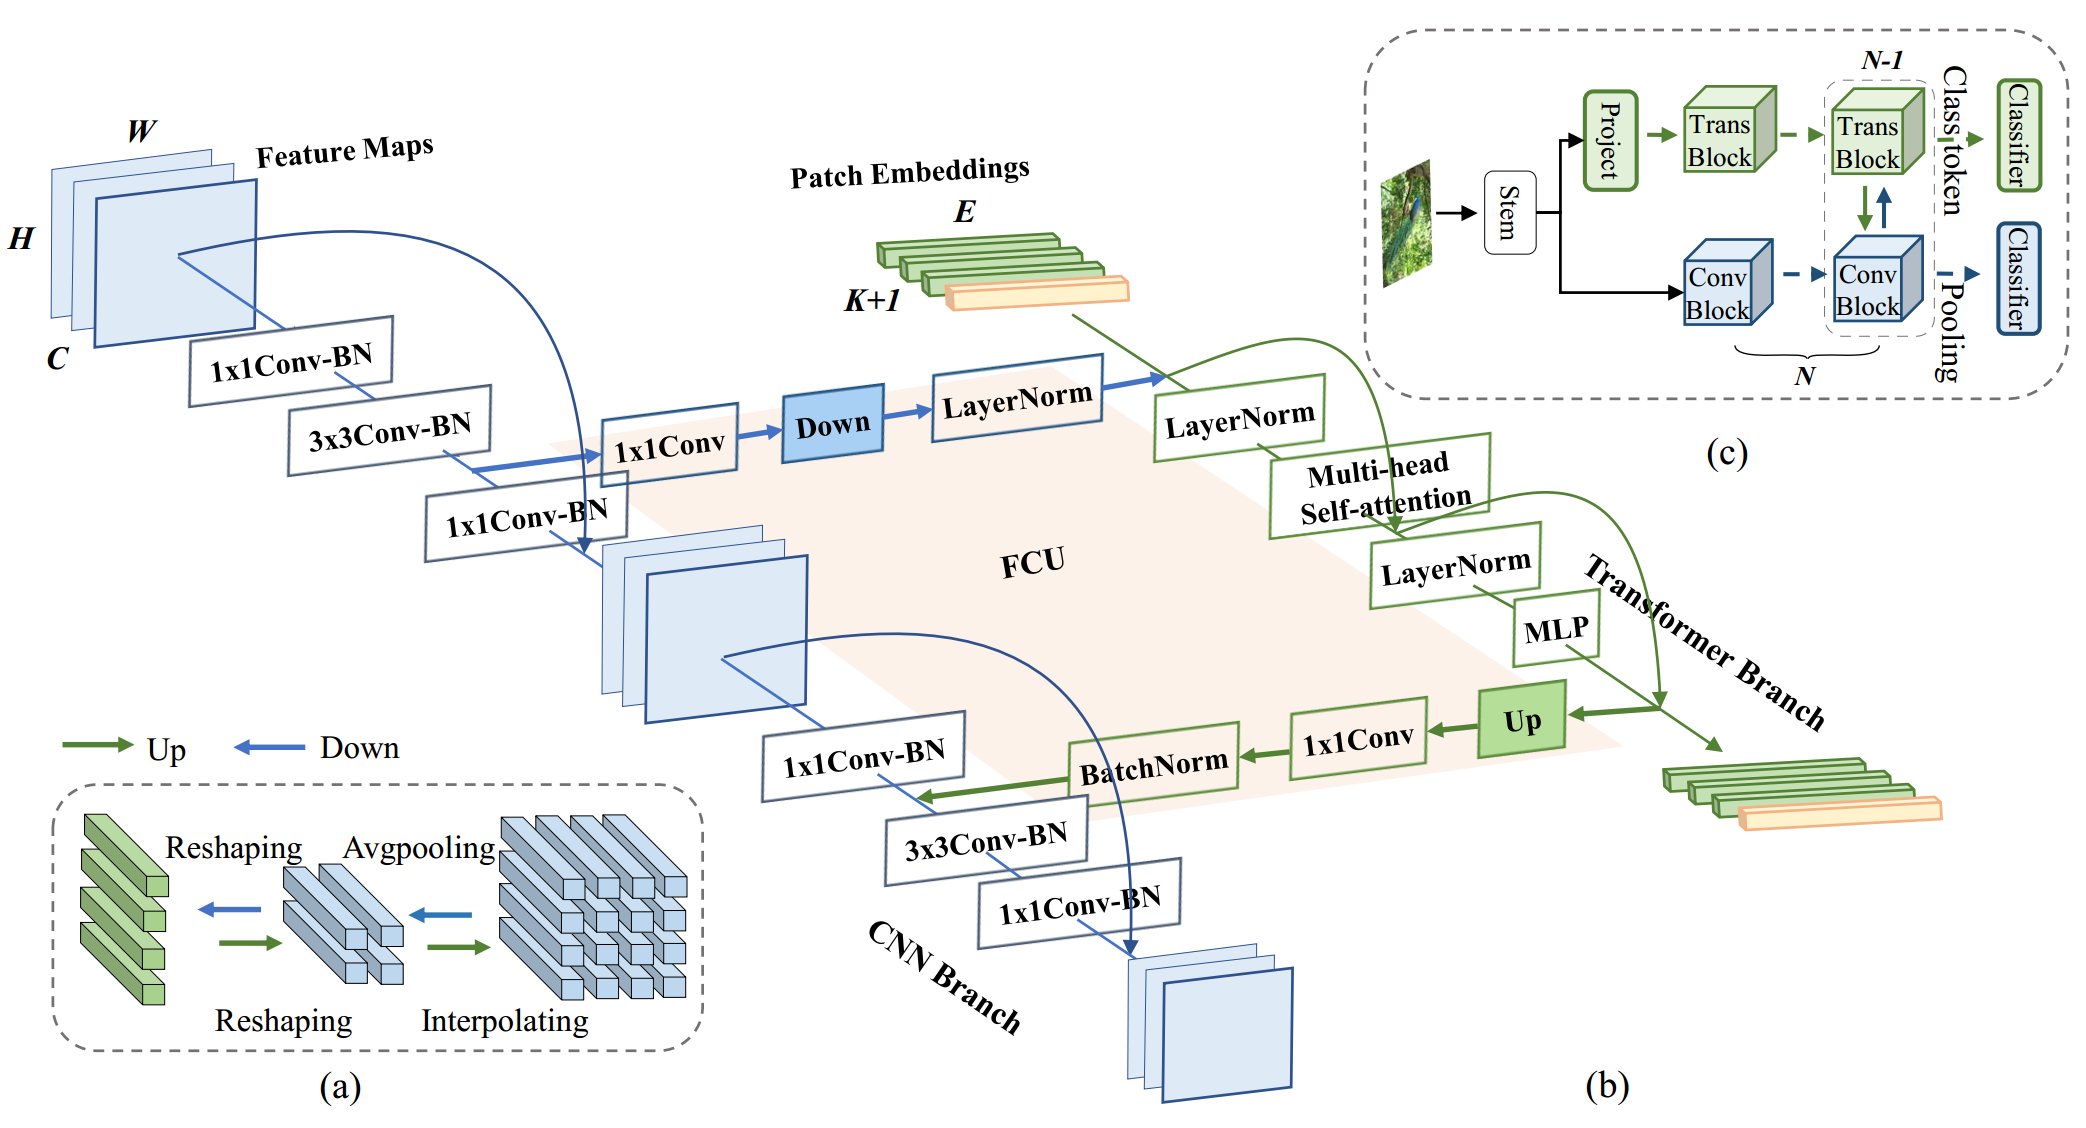
\includegraphics[width=\linewidth]{picture/LLIE/Conformer/the proposed Conformer}
				\captionsetup{font=scriptsize}
				\label{fig: Conformer}	
				\caption*{Conformer}
			\end{minipage}
			\captionsetup{font=scriptsize}
			\caption{
				\label{fig: Conformer contribution}
				Network architecture of the proposed Conformer.
			}
		\end{figure}
		
	\end{frame}
	
	\section{研究内容}
	
	\subsection{总体模型架构}
	
	\begin{frame}
		
		{\zihao{-5} \yahei 我们的研究侧重于构建一个整体恢复框架,该框架利用边缘图、初步恢复图和通道信息的融合,以提高弱光图像的质量。}
		
		% Our study focuses on constructing an overall recovery framework that utilizes the fusion of edge maps, preliminary recovery maps, and channel information to improve the quality of low-light images.
		
		% 我们的研究侧重于构建一个整体恢复框架,该框架利用边缘图、初步恢复图和通道信息的融合,以提高弱光图像的质量。我们将继续探索合适的增强网络结构,以便进一步提升恢复结果的性能。这一研究旨在为弱光图像恢复领域提供新的理论和方法,以及改善图像质量并拓展应用领域。
		
		\begin{figure}
			\begin{minipage}{.4\columnwidth}
				\begin{itemize}\zihao{-5}
					\item \textbf{初步恢复图像的生成模型}
					
					{\zihao{6} 基于 Conformer 结构}
					%\small Drawing on the conformer parallel structure, CNN branched Res-Net structure is modified to the U-Net structure.
					
					
					%我们受到了 Conformer 结构的启发,在卷积神经网络 (CNN) 中,卷积操作擅长提取局部特征,但难以捕获全局表示。Conformer 是一种混合网络结构,包含了混合网络结构,包含了并行的 CNN 分支和 Transformer 分支,其通过特征耦合模块融合局部与全局特征,目的在于不损失图像细节的同时捕捉图像全局信息。我们借鉴 Conformer 并发结构,将其中 CNN 分支的 ResNet 结构修改为 U-Net 结构。基于这一点,我们设计了一种结合U-Net 与Transformer 网络的并行模型(PACUT, Parallel architecture combining u-net and transformer)。这一模型旨在从弱光图像中提取长距离和短距离特征,以便更全面地捕捉图像的信息。通过特定的特征融合策略,我们期望能够得到初步恢复的图像。
					
					\item \textbf{边缘检测网络}
					% 弱光图像边缘生成网络
					
					{\zihao{6} 多曝光架构}
					% 多曝光架构
					
					{\zihao{6} 融合HOG和LBP图像}
					% HOG 和 LBP 融合
					
					
					\item \textbf{边缘图像指导恢复网络}
					% 边缘图像指导恢复网络
					
					{\zihao{6} 串联融合}
					% 串联融合
					
					\item \textbf{挑战}
					
					{\zihao{6} 整体模型的协调性}
					% 整体模型的协调性
					
					{\zihao{6} 消融实验的设计}
					% 消融实验
				\end{itemize}
			\end{minipage}
			\begin{minipage}{.58\columnwidth}
				\setlength{\abovecaptionskip}{-0.05cm}
				\centering 
				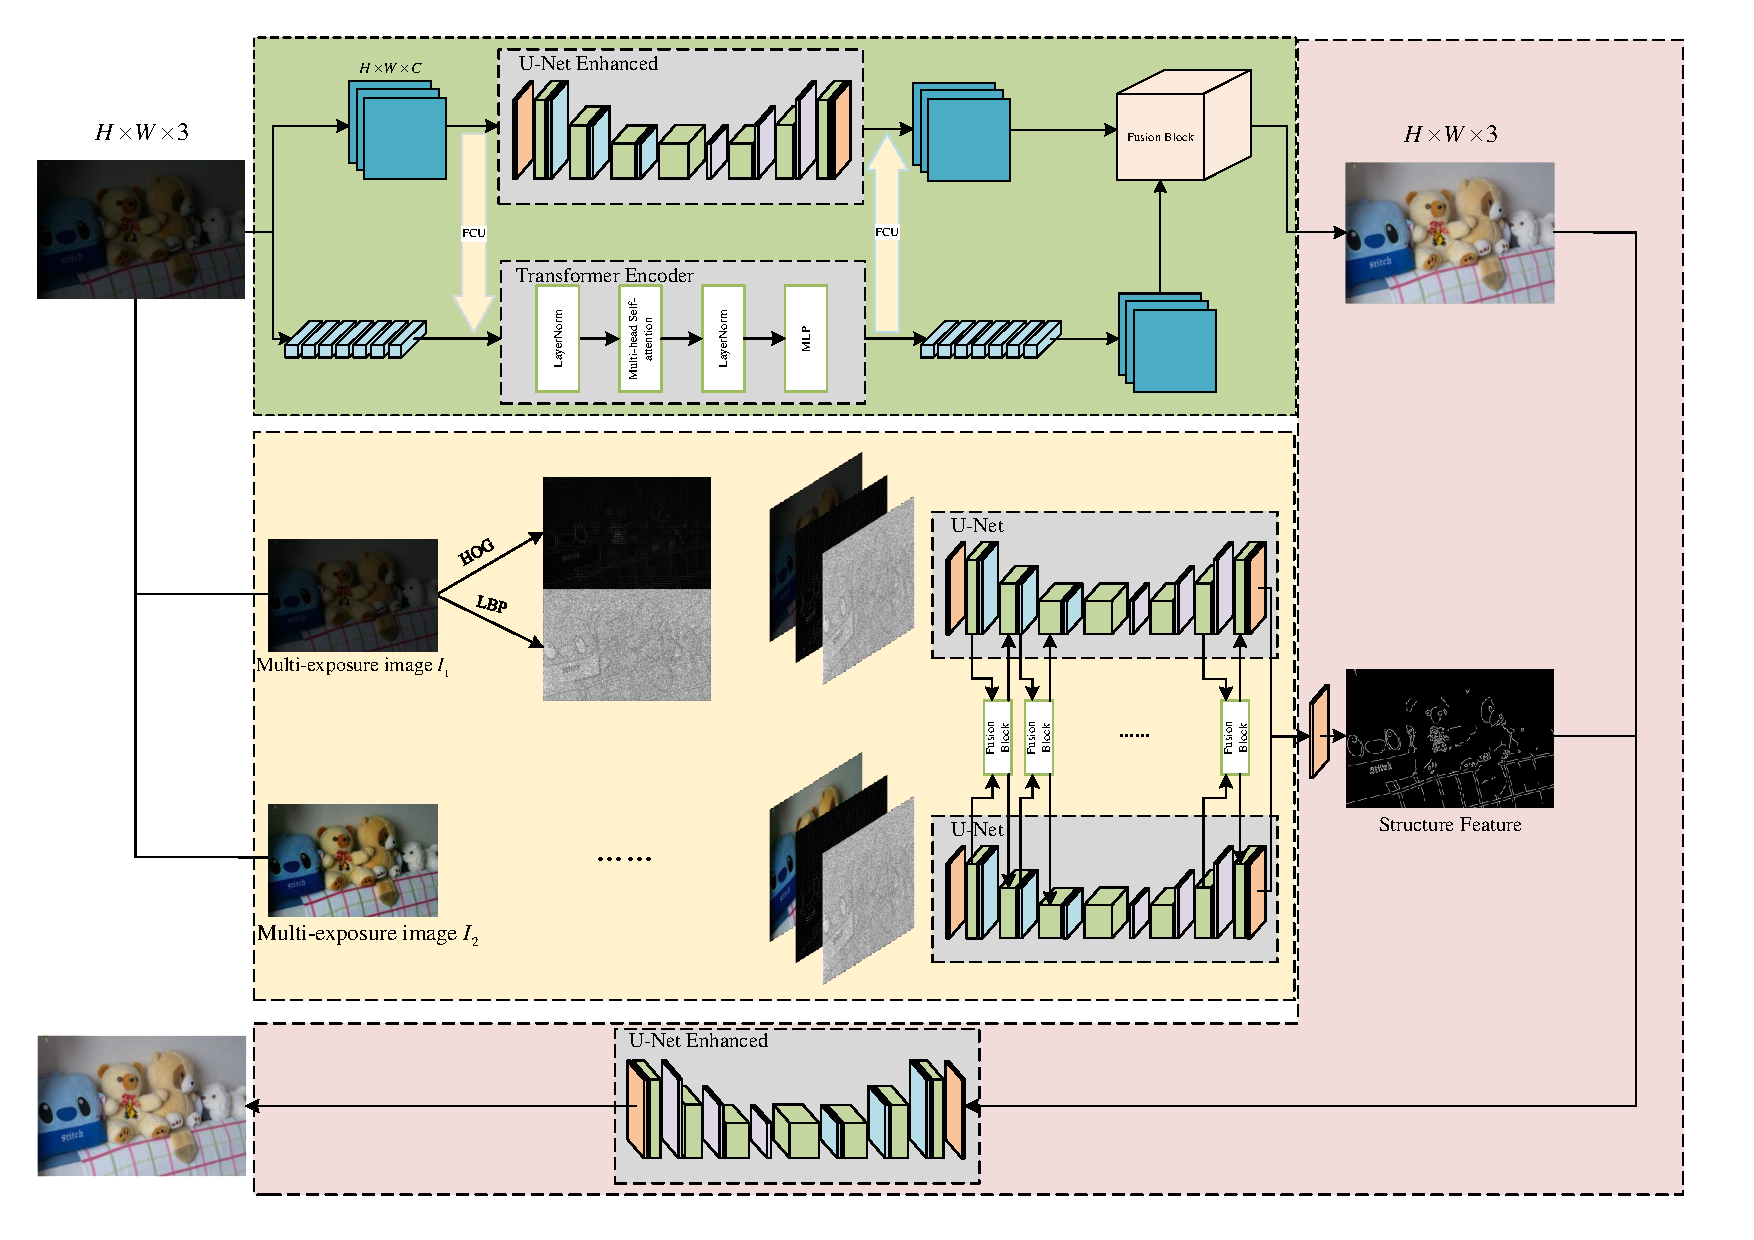
\includegraphics[width=\textwidth]{picture/LLIE/My Architecture/Total architecture}
				\captionsetup{font=scriptsize}
				\caption{
					\label{fig: Total architecture}
					Total Architecture
				}
			\end{minipage}
		\end{figure}
		
	\end{frame}
	
	
	\subsection{初步恢复图像的生成模型}
	
	\begin{frame}
		\begin{figure}
			\centering
			\begin{minipage}{.4\textwidth}
				\centering
				\small
				% 在当前的研究中,我们提出了一种新型的深度学习架构,命名为 PACUT ,旨在解决低光照条件下的图像增强问题。该模型结合了经典的 U-Net 架构和 Transformer 深度学习方法,在弱光图像增强任务中,提高恢复图像的可视性和质量,同时保留重要的细节和纹理信息。此分支的设计旨在处理图像的低级特征,如边缘、纹理和颜色信息。
				\begin{itemize} 
					\item \textbf{Abstract}
					
					\item[\checkmark]\small Based Conformer
					
					\item[\checkmark]\small Long-and short-distance feature
					
				\end{itemize}
				\begin{itemize} 
					\item \textbf{Key improvements}
					
					\item[\checkmark]\small CNN Branch
					
					% 深度卷积网络(CNN)分支:该分支基于 U-Net 架构,采用多层卷积神经网络,通过逐层提取图像的局部特征来增强图像的细节和纹理。
					
					\item[\checkmark]\small Feature Coupling Unit
					
					% 特征耦合单元(FCU):为了有效地融合 CNN 分支和 ViT 分支的特征,引入了特征耦合单元(FCU)。FCU 通过下采样(FCUDown) 和上采样(FCUUp) 操作,实现了CNN特征图和Transformer patch embeddings 之间的无缝转换,从而实现了局部特征和全局表示的连续耦合。
				\end{itemize}
				\captionsetup{font=scriptsize}
				\label{fig: Abstract}
				%\caption*{Contribution}
			\end{minipage}
			\begin{minipage}{.58\textwidth}
				\centering
				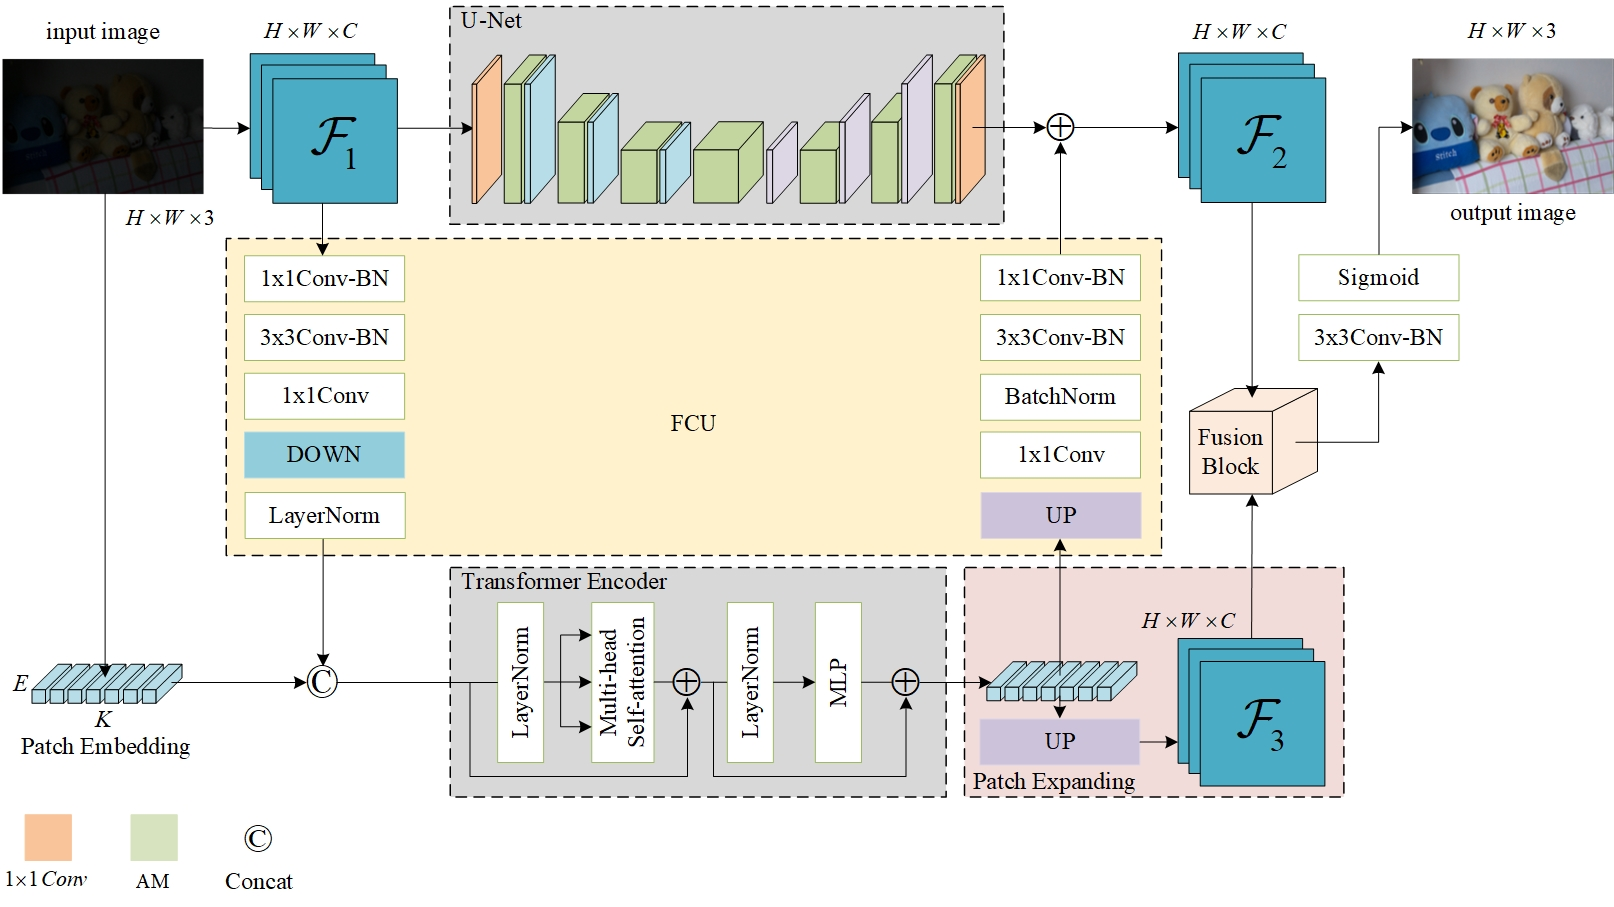
\includegraphics[width=.88\linewidth]{picture/LLIE/My Architecture/The proposed initial architecture.jpg}
				\captionsetup{font=scriptsize}
				\label{fig: PACUT}	
				\caption*{\tiny 初步恢复图像的生成模型}
			\end{minipage}\\
			\hfill
			\begin{minipage}{.28\textwidth}
				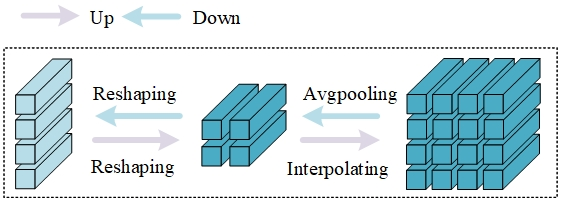
\includegraphics[width=.88\linewidth]{picture/LLIE/My Architecture/Up-sampling and down-sampling.jpg}
				\captionsetup{font=scriptsize}
				\label{fig: Up-sampling and down-sampling}	
				\caption*{\tiny Up-sampling and down-sampling}
			\end{minipage}
			\begin{minipage}{.28\textwidth}
				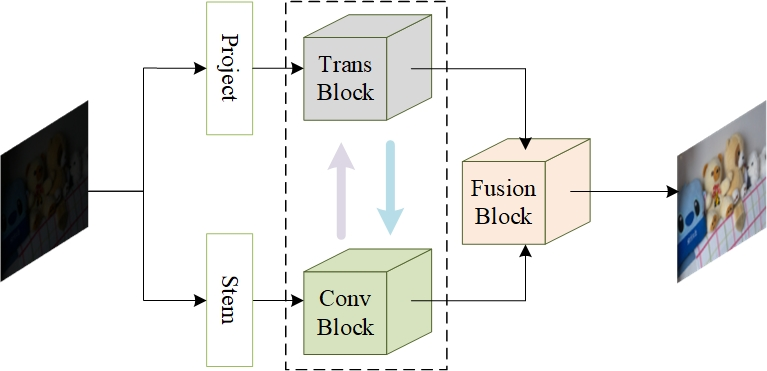
\includegraphics[width=.88\linewidth]{picture/LLIE/My Architecture/The proposed initial architecture(Abstract Picture).jpg}
				\captionsetup{font=scriptsize}
				\label{fig: The proposed initial architecture(Abstract Picture)}	
				\caption*{\tiny Thumbnail of PACUT}
			\end{minipage}
			\captionsetup{font=scriptsize}
			\caption{
				\label{fig: Parallel architecture combining u-net and transformer}
			}
		\end{figure}
		
	\end{frame}
	
	\begin{frame}
		
		\begin{itemize} 
			\item \textbf{CNN Branch}
			
			\small The foundation of the CNN branch is the U-Net structure, a network architecture designed specifically for image segmentation tasks, but also outstanding in the field of image enhancement.
			% CNN 分支的基础是 U-Net 结构,这是一种专门为图像分割任务设计的网络架构,但在图像增强领域也表现出色。U-Net 的特点是其对称的编码器-解码器结构,以及编码器和解码器之间的跳跃连接。CNN 分支的目标是从输入的弱光图像(LLI) 中提取丰富的特征,包括边缘、纹理、颜色、亮度信息,并最终输出增强的图像(EI)。
			
			\checkmark \small UNetEnhanced Method
			% UNetEnhanced 模型是一种针对低光照图像增强任务设计的深度学习架构。该模型基于经典的U-Net 架构,并引入了多项改进,以提高对低光照环境下图像的处理能力。这些改进包括更深的网络结构、改进的特征融合机制和高效的信息传递路径。
		\end{itemize}
		
		% UNetEnhance 模型由两个部分组成:1) 编码器子网络(Encoder subnetworker),2) 解码器子网络(Decoder subnetworker)。对于编码器子网络,UNetEnhance 采用了多层卷积网络,在每层中我们添加了集成模块,在集成模块中又添加了空间注意力机制和通道注意力机制。与传统 U-Net 相比,这一设计增加了网络的深度,从而能够捕获更加丰富的特征信息。我们通过引入更多的卷积层,使得模型能够在更深的层次上理解图像内容。解码器部分采用了上采样和卷积操作,以逐步恢复图像的空间分辨率。
		
		% 在这一过程中,引入了改进的特征融合策略,将编码器中的低级特征与解码器的高级特征有效结合,从而更好地重建图像细节。同时,UNetEnhance 模型在跳跃连接的设计上进行了优化,以更有效地传递编码器中的特征信息到编码器。这些连接不仅帮助保留了在下采样过程中可能丢失的细节信息,还增强了网络的特征重建能力。此外,模型的输出层经过特别设计,以确保输出图像在视觉上的质量和连贯性,我们通过准确的调整解码器子网络中的卷积操作,将解码器的输出转换为与原始输入图像相同尺寸的增强图像。
		
		\begin{figure}
			\centering
			\begin{minipage}{.65\textwidth}
				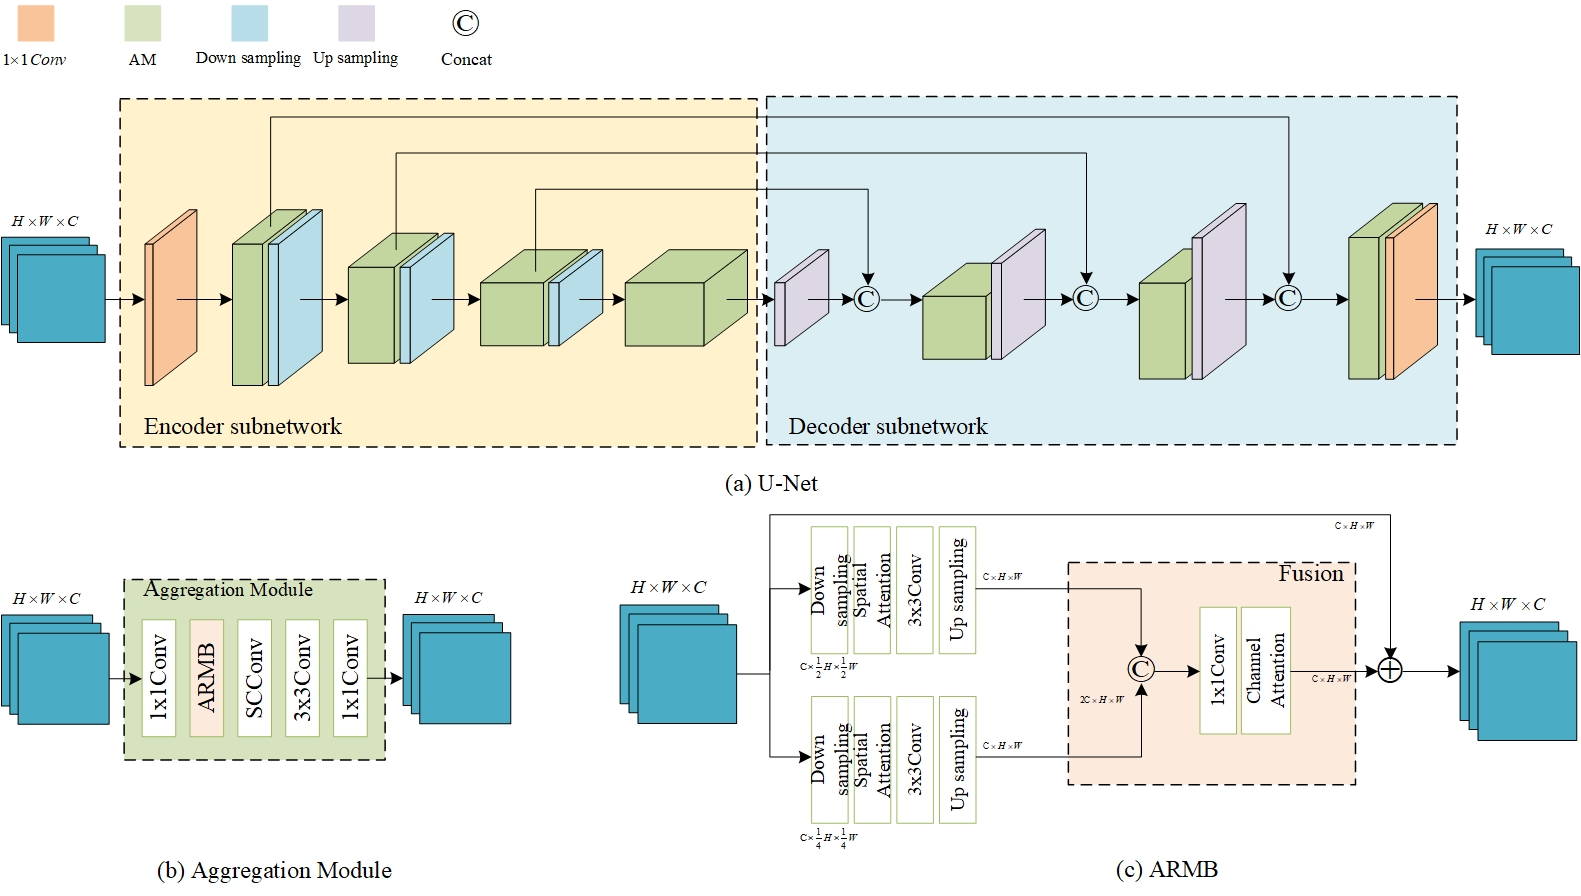
\includegraphics[width=0.85\linewidth]{picture/LLIE/My Architecture/U-Net and AM.jpg}
				\captionsetup{font=scriptsize}
				\label{fig: U-Net and AM}	
				\caption*{UNetEnhanced Method}
			\end{minipage}
			\captionsetup{font=scriptsize}
			\caption{
				\label{fig: CNN Branch}
			}
		\end{figure}
		
	\end{frame}
	
	\begin{frame}	
		
		Assuming that $I_{LLI}$ represents the input low-light image and $I_{EI}$ represents the enhanced image of the output. The operation of the encoder subnetwork $\mathcal{E}$ and the decoder subnetwork $\mathcal{D}$ can be expressed as:
		% 假设ILLI 表示输入的弱光图像,IEI 表示输出的增强图像。编码器子网络 E 和解码器子网络 D 的操作可以表示为:
		\begin{block}{UNetEnhanced}
			\begin{equation}
				\begin{aligned}
					I_{EI} = \mathcal{D} \left( \mathcal{E} \left( I_{LLI} \right) \right)
				\end{aligned}
				\label{eq: UNetEnhance model}
			\end{equation}
		\end{block}
		
		\begin{block}{Aggregation Module}
			\begin{equation}
				\begin{aligned}
					\text{AM}_{i}(x) = f^{1 \times 1} \left(f^{3 \times 3} \left(\text{SCConv}\left( \text{ARMB} \left( f^{1 \times 1} (x)\right)\right)\right)\right)
				\end{aligned}
			\end{equation}
		\end{block}
		
		Where $f ^ {1 \times 1} $ is the $1 \times 1$ convolution layer, and the operation of ARMB and SCConv depends on their internal structure.
		% 其中,f1×1为1 × 1 卷积层,ARMB 和SCConv 的操作依据其内部结构进行。
	\end{frame}
	
	\begin{frame}	
		
		ARMB (Attention Residual Merging Block) 
		
		% ARMB (Attention Residual Merging Block) 是一种用于深度学习模型中的结构单元,特别是在处理图像相关任务时,它的主要作用是融合来自不同来源的特征,并通过注意力机制增强模型对关键信息的关注。其核心作用之一是融合来自模型不同层或不同分支的特征。
		
		Suppose $ \mathcal {F} _ {in} $ is the input feature graph, $ \mathcal {F} _ {out} $ is the output feature graph, $ \mathcal {F} _ {i} ^ \prime$ means that the feature graph is trimmed or enlarged, see the following equation:
		
		% 假设Fin 是输入特征图,Fout 是输出特征图,F′i 表示对特征图进行裁剪或放大,见下式:
		
		\begin{block}{ARMB}
			\begin{equation}
				\begin{aligned}
					&\mathcal{F}^\prime_{\frac{1}{2}} = \text{Resize}\left(\mathcal{F}_{in},\left(\frac{H}{2},\frac{W}{2}\right)\right), \\
					&\mathcal{F}^\prime_{\frac{1}{4}} = \text{Resize}\left(\mathcal{F}_{in},\left(\frac{H}{4},\frac{W}{4}\right)\right), \\
					&\mathcal{F}_{out} = W_1\mathcal{F}_{out} + W_2\mathcal{C} \left( f^{1 \times 1}  \left[\mathcal{F}^\prime_2 (f^{3 \times 3}(\mathcal{S}(\mathcal{F}^\prime_{\frac{1}{2}}))), \mathcal{F}^\prime_4 (f^{3 \times 3}(\mathcal{S}(\mathcal{F}^\prime_{\frac{1}{4}})))\right] \right).
				\end{aligned}
				\label{eq: ARMB}
			\end{equation}
		\end{block}
		
		Where $ \mathcal{S} $ and $ \mathcal{C} $ represent the spatial and channel attention function, respectively, and $W_1$ and $W_2$ are the corresponding feature graph weights.
		
		% 其中S 和 C 分别表示空间注意力函数和通道注意力函数,W1 和W2 为对应的特征图权重。
	\end{frame}
	
	\begin{frame}
		\begin{figure}
			\centering
			\begin{minipage}{.45\textwidth}
			\begin{itemize} 
				\item \textbf{Transformer Branch}
				
				Based Vision Transformer (ViT)
				
				Extract global features
				% 这一分支的目标是捕获图像中的长距离依赖关系,以辅助CNN 分支的局部特征提取。
				
			\end{itemize}
			
	
			\begin{itemize} 
				\item \textbf{Patch Embedding}
				% Patch Embedding是一种常见的操作,它将图像分割成更小的块(patches),然后将这些块转换成一系列的向量,这些向量可以被用作模型的输入。
				
				\item[\checkmark] Segmenting
				
				\item[\checkmark] Reshape
				
				\item[\checkmark] Flatten
				
				\item[\checkmark] Linear Projection
				
			\end{itemize}
			\end{minipage}
			\begin{minipage}{.45\textwidth}
				\includegraphics[width=0.85\linewidth]{picture/LLIE/My Architecture/Patch Embedding}
				\captionsetup{font=scriptsize}
				\caption*{Patch Embedding}
			\end{minipage}
			\captionsetup{font=scriptsize}
			\caption*{
				\label{fig: Patch Embedding}
			}
		\end{figure}
	\end{frame}

	\begin{frame}
		\begin{figure}
			\centering
			\begin{minipage}{.95\textwidth}
				\includegraphics[width=\linewidth]{picture/LLIE/My Architecture/Patch Embedding(ViT)}
				\captionsetup{font=scriptsize}
				\caption{Patch Embedding in Transformer Branch}
			\end{minipage}
			\captionsetup{font=scriptsize}
			\caption*{
				\label{fig: Patch Embedding in ViT}
			}
		\end{figure}
	\end{frame}
	
	\begin{frame}
		\begin{itemize} 
			\item \textbf{Feature Coupling Unit}
			% CNN 分支中特征映射和Transformer 分支中patch embedding,如何消除他们之间的错误是一个重要的问题,为了解决这个问题,使用FCU 以交互的方式将局部特征和全局表示进行连续耦合。
			
			Feature mapping in CNN branch and patch embedding in Transformer branch, how to eliminate errors between them is an important question, and to solve this problem, the FCU is used to continuously couple local features and global representations in an interactive manner.
			
			\item[\checkmark] CNN dim: $H \times W \times C$
			
			\item[\checkmark] Transformer dim: $K \times D$
			% 其中K, D分别表示图像 patch 的数量和 embedding 的维度。用于分类的 Vision Transformer 模型中 patch embedding 的形状为 (K + 1)×D,其中 1 为类别嵌入 (Class Token),但是在 Transformer 分支中,我们去除了类别嵌入。			
			
			% 特征映射和patch embedding 之间存在显著的语义鸿沟,即特征映射是从局部卷积算子收集的,而 patch embedding 则是通过自注意力机制聚合的,所以通过应用 FCU 可以填补语义空白。 
		\end{itemize}
	\end{frame}
	
	\subsection{边缘检测网络}
	
	\begin{frame}
		
		{\zihao{6} \yahei Liu\textcolor{blue}{\citep{liu2017richer}}发现不同卷积层获得的结果随着深度增加而更加粗糙,其提出 RCF(Richer convolutional features) 方法充分利用所有 CNN 层的结果。}
		
		\begin{figure}
			\centering
			\setlength{\abovecaptionskip}{-0.05cm} 		
			\begin{minipage}{0.11\columnwidth}
				\includegraphics[width=\linewidth]{picture/LLIE/RCF/origin image}
				\caption*{\tiny (a) origin image}
				\label{fig: origin image}
			\end{minipage}
			\begin{minipage}{0.11\columnwidth}
				\includegraphics[width=\linewidth]{picture/LLIE/RCF/GT}
				\caption*{\tiny (b) GT}
				\label{fig: RCF_GT}
			\end{minipage}
			\begin{minipage}{0.11\columnwidth}
				\includegraphics[width=\linewidth]{picture/LLIE/RCF/conv3_1}
				\caption*{\tiny (c) conv3\_1}
				\label{fig: conv3_1}	
			\end{minipage}
			\begin{minipage}{0.11\columnwidth}
				\includegraphics[width=\linewidth]{picture/LLIE/RCF/conv3_2}
				\caption*{\tiny (d) conv3\_2}
				\label{fig: conv3_2}	
			\end{minipage}
			\begin{minipage}{0.11\columnwidth}
				\includegraphics[width=\linewidth]{picture/LLIE/RCF/conv3_3}
				\caption*{\tiny (e) conv3\_3}
				\label{fig: conv3_3}
			\end{minipage}
			\begin{minipage}{0.11\columnwidth}
				\includegraphics[width=\linewidth]{picture/LLIE/RCF/conv4_1}
				\caption*{\tiny (f) conv4\_1}
				\label{fig: conv4_1}
			\end{minipage}
			\begin{minipage}{0.11\columnwidth}
				\includegraphics[width=\linewidth]{picture/LLIE/RCF/conv4_2}
				\caption*{\tiny (g) conv4\_2}
				\label{fig: conv4_2}	
			\end{minipage}
			\begin{minipage}{0.11\columnwidth}
				\includegraphics[width=\linewidth]{picture/LLIE/RCF/conv4_3}
				\caption*{\tiny (h) conv4\_3}
				\label{fig: conv4_3}	
			\end{minipage}
			\caption{
				\tiny 建立了一个基于 VGG16\cite{simonyan2014very} 的简单网络来产生侧输出(c-h)。我们可以看到,卷积特征逐渐变得更粗,而中间层(c、d、f、g)包含了在其他层中没有出现的基本细节。
			}
		\end{figure}
		
		{\zihao{6} \yahei 相比之下,HED (Holistically-nested edge detection) \textcolor{blue}{\cite{xie2015holistically}}方法仅采用了 VGG16 架构中每个阶段的最后一层卷积输出,而 RCF (Richer Convolutional Features) 方法则利用了每个层级的卷积结果。}
		
	\end{frame}
	
%	\begin{frame}
%		
%		\begin{itemize} 
%			\item \textbf{Traditional Method}
%			% 获取图像边缘的深度学习方法主要依赖于卷积神经网络(CNN)的变体和架构,这些方法能够有效地提取图像的特征,包括边缘信息。以下是一些常见的深度学习方法,用于获取图像边缘。
%			
%			CNN
%			% 传统的CNN架构,如LeNet、AlexNet、VGGNet等,可以通过训练来识别图像边缘。在这些网络的初级层中,通常会学习到类似于传统边缘检测滤波器(如 Sobel 或 Canny)的特征。
%			
%			Auto-encoder
%			% 自编码器可以用于学习图像的压缩表示,其中编码器部分可以被训练来提取图像的边缘信息。
%			
%			GANS
%			% GANs可以用于边缘检测,特别是在图像到图像的转换任务中
%			
%			U-Net
%			% U-Net是一种流行的用于图像分割的网络架构,它也可以被用于边缘检测。U-Net的对称结构和跳跃连接特别适合于捕捉图像的细节和边缘。
%		\end{itemize}
%		\begin{itemize} 
%			\item \textbf{Challenge}
%			
%			Processing dark light images directly can distort the edge map
%			% 直接处理暗光图片会使得边缘图失真
%			
%		\end{itemize}
%	\end{frame}
	
	\begin{frame}
		\begin{figure}
			\centering
			\setlength{\abovecaptionskip}{-0.05cm} 	
			\begin{minipage}{.19\textwidth}
				\centering
				\includegraphics[width=\linewidth]{picture/LLIE/My Architecture/Edge Detection/low00044}
				\caption*{\tiny LLI}
				\label{fig: LLI}
			\end{minipage}
			\begin{minipage}{.19\textwidth}
				\centering
				\includegraphics[width=\linewidth]{picture/LLIE/My Architecture/Edge Detection/low00044_canny}
				\caption*{\tiny LLI Canny}
				\label{fig: LLI_canny}
			\end{minipage}
			\begin{minipage}{.19\textwidth}
				\centering
				\includegraphics[width=\linewidth]{picture/LLIE/My Architecture/Edge Detection/low00044_rcf}
				\caption*{\tiny LLI RCF}
				\label{fig: LLI_rcf}	
			\end{minipage}
			\begin{minipage}{.19\textwidth}
				\centering
				\includegraphics[width=\linewidth]{picture/LLIE/My Architecture/Edge Detection/low00044_hog}
				\caption*{\tiny LLI HOG}
				\label{fig: LLI_hog}	
			\end{minipage}
			\begin{minipage}{.19\textwidth}
				\centering
				\includegraphics[width=\linewidth]{picture/LLIE/My Architecture/Edge Detection/low00044_lbp}
				\caption*{\tiny LLI LBP}
				\label{fig: LLI_lbp}	
			\end{minipage}
			\begin{minipage}{.19\textwidth}
				\centering
				\includegraphics[width=\linewidth]{picture/LLIE/My Architecture/Edge Detection/normal00044}
				\caption*{\tiny GT}
				\label{fig: GI}
			\end{minipage}
			\begin{minipage}{.19\textwidth}
				\centering
				\includegraphics[width=\linewidth]{picture/LLIE/My Architecture/Edge Detection/normal00044_canny}
				\caption*{\tiny GT Canny}
				\label{fig: GT_canny}	
			\end{minipage}
			\begin{minipage}{.19\textwidth}
				\centering
				\includegraphics[width=\linewidth]{picture/LLIE/My Architecture/Edge Detection/normal00044_rcf}
				\caption*{\tiny GT RCF}
				\label{fig: GT_rcf}	
			\end{minipage}
			\begin{minipage}{.19\textwidth}
				\centering
				\includegraphics[width=\linewidth]{picture/LLIE/My Architecture/Edge Detection/normal00044_hog}
				\caption*{\tiny GT HOG}
				\label{fig: GT_hog}	
			\end{minipage}
			\begin{minipage}{.19\textwidth}
				\centering
				\includegraphics[width=\linewidth]{picture/LLIE/My Architecture/Edge Detection/normal00044_lbp}
				\caption*{\tiny GT LBP}
				\label{fig: GT_lbp}	
			\end{minipage}
			\captionsetup{font=scriptsize}
			\caption{
				\label{fig: LLI Structure Information}
				LLI and GT Structure Information
			}
		\end{figure}
		
		\vspace{-0.5cm}
		
		{\zihao{6} \yahei 传统方法如 Canny 和 Sobel 算子\textcolor{blue}{\cite{maini2009study}}在直接从低光照图像中提取边缘时面临较大挑战。然而,基于深度学习的方法能从低光照图像中提取出更为详细的边缘图像,虽然与真实边缘仍有差异。我们的研究目标是缩减这一差距,以提高基于结构建模指导的模型的准确性。}
	\end{frame}
	
	\begin{frame}
		
		\begin{itemize}\zihao{5}
			\item \textbf{方向梯度直方图, HOG}
			\vspace{.3cm}
			% 一般而言,HOG特征在物体检测(特别是行人检测)中非常有效,它通常与支持向量机(SVM)分类器一起使用。
			% HOG 主要原理是计算图像的梯度幅值和方向。具体来说先把图像分割个小的连续区域(Cell),计算每一个区域梯度方向的直方图,最后合并成更大的区域(Block) 来对直方图进行归一化,然后合并所有 Block 形成最终的 HOG 特征图。		
			
			%\small HOG is a feature control for shape information and texture information for local images.
			\checkmark {\zihao{6} HOG 是一个用于局部图像的形状信息和纹理信息的特征控件。它基于图像的梯度方向来构建直方图。}
			
			%\small Vectors of the shape and edge information of the object in the image
			\checkmark {\zihao{6} HOG特征表示包含图像中对象的形状和边缘信息的向量,它分析了图像中局部梯度方向的分布。}
			
			%\small HOG maintains good invariance to both image geometry and optical deformation.
			\checkmark {\zihao{6} 由于HOG是在图像的局部方格单元上操作,所以它对图像几何的和光学的形变都能保持很好的不变性。}
		\end{itemize}
		
		\begin{itemize} \zihao{5}
			\item \textbf{局部二值模式图, LBP}
			\vspace{.3cm}
			% 一般而言,HOG特征在物体检测(特别是行人检测)中非常有效,它通常与支持向量机(SVM)分类器一起使用。
			% HOG 主要原理是计算图像的梯度幅值和方向。具体来说先把图像分割个小的连续区域(Cell),计算每一个区域梯度方向的直方图,最后合并成更大的区域(Block) 来对直方图进行归一化,然后合并所有 Block 形成最终的 HOG 特征图。		
			
			%\small LBP is an operator used to describe the local features of images
			\checkmark {\zihao{6} LBP 是一种用来描述图像局部特征的算子。}
			
			%\small LBP features have significant advantages such as gray invariance and rotation invariance.
			\checkmark {\zihao{6} LBP特征具有灰度不变性和旋转不变性等显著优点.}
			
			%\small HOG maintains good invariance to both image geometry and optical deformation.
			% LBP主要工作原理如下:对于图像中的每个像素,考虑其周围的一个领域(例如,3 × 3 的窗口),然后将邻域中的每个像素与中心像素进行比较。如果领域像素的值大于或等于中心像素的值,则将其标记为1,否则标记为0。这样相邻的所有域都会产生一个二进制模式(例如,11100101),通过计算所有二进制模式的直方图作为图像的 LBP 特征。
		\end{itemize}
		
		\begin{itemize} \zihao{5}
			\item \textbf{我们能从 HOG 和 LBP获得什么?}
			\vspace{.3cm}
			
			%\small Edge information
			\checkmark {\zihao{6} 边缘信息}
			
			%\small Necessarily Work?
			\checkmark {\zihao{6} 是否一定有效?}
			
			%\small How to solve?
			\checkmark {\zihao{6} 怎么利用这两个特征?}
		\end{itemize}
	\end{frame}
	
	\begin{frame}
		\begin{figure}
			\centering
			\setlength{\abovecaptionskip}{-0.005cm} 	
			\begin{minipage}{.3\textwidth}
				\centering
				\includegraphics[width=\linewidth]{picture/LLIE/My Architecture/Edge Detection/low00269}
				\caption*{\small LLI with noise}
			\end{minipage}
			\begin{minipage}{.3\textwidth}
				\centering
				\includegraphics[width=\linewidth]{picture/LLIE/My Architecture/Edge Detection/low00269_hog}	
				\caption*{\small LLI HOG}
			\end{minipage}
			\begin{minipage}{.3\textwidth}
				\centering
				\includegraphics[width=\linewidth]{picture/LLIE/My Architecture/Edge Detection/low00269_lbp}	
				\caption*{\small LLI LBP}
			\end{minipage} \\
			\vspace{-0.3cm}
			\begin{minipage}{.3\textwidth}
				\centering
				\includegraphics[width=\linewidth]{picture/LLIE/My Architecture/Edge Detection/normal00269}
				\caption*{\small GT}
			\end{minipage}
			\begin{minipage}{.3\textwidth}
				\centering
				\includegraphics[width=\linewidth]{picture/LLIE/My Architecture/Edge Detection/normal00269_hog}
				\caption*{\small GT HOG}
			\end{minipage}
			\begin{minipage}{.3\textwidth}
				\centering
				\includegraphics[width=\linewidth]{picture/LLIE/My Architecture/Edge Detection/normal00269_lbp}
				\caption*{\small GT LBP}
			\end{minipage}
			\caption{
				\label{fig: LLI Structure Information1}
				\small LLI with noise and GT Structure Information
			}
		\end{figure}
	\end{frame}
	
	\begin{frame}
		\begin{figure}
			\centering
			\setlength{\abovecaptionskip}{-0.05cm} 	
			\begin{minipage}{0.9\textwidth}
				\centering
				\includegraphics[width=\linewidth]{picture/LLIE/My Architecture/Edge Detection Network}
				\captionsetup{font=scriptsize}
				\label{fig: Edge Detection Network}	
				\caption{Edge Detection Network}
			\end{minipage}
		\end{figure}
		
		\vspace{-0.5cm}
		
		{\zihao{6} \yahei 本研究尝试使用不同曝光度的图片,获取它们的 HOG 和 LBP 图像,并采用多曝光图像融合架构,从而获得更接近真实边缘结构的边缘图像。}
	\end{frame}
	
	\section{具体工作内容}
	
	\subsection{已完成工作}
	
	\begin{frame}
		{\zihao{5} \yahei \textbf{已完成工作}}
		% 实验的过程中,确保所有的实验在相同的硬件和软件环境下进行,并且为了确保结果的可靠性,可能需要多次运行实验并取平均值。我们主要基于 PyTorch 进行模型的搭建、训练和评估,使用 Matplotlib 库用于绘制图标和注意力图。基于scikit-image 库计算PSNR、SSIM 等评价指标。
		
		{\zihao{-5} \yahei 我们针对初步恢复图像的生成模型进行了实验验证,以验证所提出方法的有效性。}
		
		\begin{itemize}\zihao{-5}
			\item [(1)] 首先,介绍了实验的具体实施细节,包括网络的实现、所采用的数据集以及评估指标的选择。
			\item [(2)] 接着,通过与当前领先技术的比较分析,展示了我们网络在低光图像增强任务中的性能优势。
			\item [(3)] 最后,为了深入理解各个网络组件的贡献,我们执行了一系列消融研究,探讨了这些组件在低光图像增强任务中的作用和重要性。
		\end{itemize}
		
	\end{frame}
	
	
	\subsubsection{数据集和评价指标}
	
	\begin{frame}
		{\zihao{-5} \yahei \textbf{数据集和评价指标}}
		% 实验的过程中,确保所有的实验在相同的硬件和软件环境下进行,并且为了确保结果的可靠性,可能需要多次运行实验并取平均值。我们主要基于 PyTorch 进行模型的搭建、训练和评估,使用 Matplotlib 库用于绘制图标和注意力图。基于scikit-image 库计算PSNR、SSIM 等评价指标。
		
		\begin{itemize} 
			\item \textbf{弱光数据集}
		\end{itemize}
		
		\begin{table}[!htbp]
			\centering
			\tiny
			%\resizebox{\textwidth}{!}{ %按照宽度调整调整表格大小
				\begin{tabular}{>{\centering\arraybackslash}m{3cm}|c|c|c|c}
					
					\hline
					
					\textbf{Name} & \textbf{Number} & \textbf{Format} & \textbf{Real/Syn} & \textbf{Video} \\
					
					\hline
					
					LOL\textcolor{blue}{\citep{wei2018deep}} & 500 & RGB & Real & \\
					
					SCIE\textcolor{blue}{\citep{cai2018learning}} & 4,413 & RGB & Real & \\
					
					VE-LOL-L\textcolor{blue}{\citep{jiang2019learning}} & 2,500 & RGB & Real+Syn & \\
					
					MIT-Adobe FiveK\textcolor{blue}{\citep{bychkovsky2011learning}} & 5,000 & Raw & Real & \\
					
					SID\textcolor{blue}{\citep{wei2018deep}} & 5,094 & Raw & Real & \\
					
					DRV\textcolor{blue}{\citep{chen2019seeing}} & 202 & Raw & Real & \checkmark  \\
					
					SMOID\textcolor{blue}{\citep{jiang2019learning}} & 179 & Raw & Real & \checkmark  \\
					
					\hline
					
				\end{tabular}
				%}
			\captionsetup{font=scriptsize} %设置标题字体与表格字体一致
			\caption{\label{tab: Paired_training_datases}
				Summary of paired training datasets. 'Syn' represents Synthetic.} %表格的标题
			
		\end{table}
		
		\vspace{-0.3cm}
		
		\begin{itemize}\zihao{5}
			\item \textbf{评价指标}
			
			\checkmark {\zihao{6} 峰值信噪比(PSNR)是应用最广泛的指标之一。PSNR值越高,失真越小。单位为dB。}
			
			\checkmark {\zihao{6} 结构相似性(SSIM)是参考图像质量评价中应用最广泛的标准。越接近1,两个图像就越相似。}
		\end{itemize}
	\end{frame}
	
	\subsubsection{对比实验和消融实验}
	
	\begin{frame}
		{\zihao{-5} \yahei \textbf{对比实验}}
		
		{\zihao{6} \yahei 我们将所提算法的结果与多个公开可获得的代码进行比较,包括HE\textcolor{blue}{\citep{pisano1998contrast}}、LightenNet\textcolor{blue}{\citep{li2018lightennet}}、LLNet\textcolor{blue}{\citep{lore2017llnet}}、Retinex-Net\textcolor{blue}{\citep{wei2018deep}}、MBLLEN\textcolor{blue}{\citep{lv2018mbllen}}、EnlightenGAN\textcolor{blue}{\citep{jiang2021enlightengan}}、Zero-DCE\textcolor{blue}{\citep{guo2020zero}}以及KinD\textcolor{blue}{\citep{zhang2019kindling}}。}
		
		\begin{table}[!htbp]
			\centering
			\tiny
			\resizebox{\textwidth}{!}{ %按照宽度调整调整表格大小
				\begin{tabular}{>{\centering\arraybackslash}m{2.5cm}|c|c|c|c|c|c}
					
					\hline %添加表格头部粗线
					
					\multirowcell{2}{\textbf{Method}} & \multicolumn{3}{c|}{\makecell{\textbf{LOL}}} & \multicolumn{3}{c}{\makecell{\textbf{SCIE}}} \\
					
					\cline{2-7}
					
					
					& \textbf{PSNR↑} & \textbf{SSIM↑} & \textbf{NIQE↓} & \textbf{PSNR↑}  & \textbf{SSIM↑} & \textbf{NIQE↓} \\
					
					\hline
					
					input & 7.773 & 0.181 & 0.560 & 17.824 & 0.779 & 0.148  \\
					
					\hline	
					
					HE             & 15.467 & 0.504 & 9.531 & 15.342 & 0.741 & 9.232 \\
					LightenNet     & 10.301 & 0.361 & 7.422 & 13.579 & 0.744 & 8.166 \\
					LLNet          & \textcolor{blue}{17.953} & 0.704 & \textcolor{red}{3.974} & 12.177 & 0.645 & 4.292 \\
					Retinex-Net    & 16.774 & 0.462 & 5.474 & 12.310 & 0.671 & 7.239 \\ 
					KinD 	          & 16.648 & \textcolor{blue}{0.779} & 6.175 & 21.103 & \textcolor{red}{0.838} & 4.195 \\
					MBLLEN         & 17.902 & 0.715 & \textcolor{blue}{4.247} & 13.638 & 0.632 & \textcolor{blue}{2.108} \\
					EnlightenGAN   & 17.483 & 0.658 & 4.889 & 18.726 & 0.822 & 5.216 \\
					Zero-DCE       & 17.622 & 0.556 & 7.972 & \textcolor{red}{22.682} & 0.810 & \textcolor{red}{1.158} \\
					\textbf{Ours}  & \textcolor{red}{22.780} & \textcolor{red}{0.823} & 4.473 & \textcolor{blue}{21.543} & \textcolor{blue}{0.835} & 3.412 \\
					\hline
					
				\end{tabular}
			}
			\captionsetup{font=scriptsize} %设置标题字体与表格字体一致
			\caption{
				\tiny LOL和SCIE数据集在各方法下的对比值,其中红色表示最优,蓝色表示次优,$↑$表示越高越好,$↓$表示越低越好。
			} 
		\end{table}
		
%		\begin{itemize}
%			\item \textbf{Performance Evaluation}
%			
%			\checkmark MSE
%			% 均方误差
%			
%			\checkmark PSNR
%			% 峰值信噪比
%			
%			\checkmark SSIM
%			% 结构相似性指数
%			
%			\checkmark LPIPS
%			% 感知图像质量评估
%		\end{itemize}
%		
%		\begin{itemize}
%			\item \textbf{Results analysis and reporting}
%			
%			\checkmark All experimental results were compiled into tables or graphs.
%			% 数据整理: 将所有实验结果整理成表格或图表。
%			
%			\checkmark Analysis of differences
%			% 分析: 分析不同数据集和不同模型配置(如有/无Transformer分支) 的性能差异。
%		\end{itemize}
				
	\end{frame}
	
	\begin{frame}
	{\zihao{-5} \yahei \textbf{对比实验}}
	
		\begin{figure}
		\centering 
		\setlength{\abovecaptionskip}{-0.05cm}
		\begin{minipage}{0.19\textwidth}
			\includegraphics[width=\linewidth]{picture/LLIE/Efficent/Input}
			\caption*{\tiny (a) Input}
			\label{fig: LLI Input}
		\end{minipage}
		\begin{minipage}{0.19\textwidth}
			\includegraphics[width=\linewidth]{picture/LLIE/Efficent/LightenNet}
			\caption*{\tiny (b) LightenNet}
			\label{fig: LightenNet}
		\end{minipage}
		\begin{minipage}{0.19\textwidth}
			\includegraphics[width=\linewidth]{picture/LLIE/Efficent/LLNet}				
			\caption*{\tiny (c) LLNet}
			\label{fig: LLI LLNet}	
		\end{minipage}
		\begin{minipage}{0.19\textwidth}
			\includegraphics[width=\linewidth]{picture/LLIE/Efficent/RetinexNet}
			\caption*{\tiny (d) RetinexNet}
			\label{fig: LLI RetinexNet}	
		\end{minipage}
		\begin{minipage}{0.19\textwidth}
			\includegraphics[width=\linewidth]{picture/LLIE/Efficent/KinD}
			\caption*{\tiny (e) KinD}
			\label{fig: KinD}	
		\end{minipage}\\
		\vspace{-0.3cm}
		\begin{minipage}{0.19\textwidth}
			\includegraphics[width=\linewidth]{picture/LLIE/Efficent/MBLLEN}
			\caption*{\tiny (f) MBLLEN}
			\label{fig: MBLLEN_contrast}	
		\end{minipage}
		\begin{minipage}{0.19\textwidth}
			\includegraphics[width=\linewidth]{picture/LLIE/Efficent/EnlightenGAN}
			\caption*{\tiny (g)EnlightenGAN}
			\label{fig: LLI EnlightenGAN}	
		\end{minipage}
		\begin{minipage}{0.19\textwidth}
			\includegraphics[width=\linewidth]{picture/LLIE/Efficent/Zero-DCE}
			\caption*{\tiny (h) Zero-DCE}
			\label{fig: Zero-DCE}	
		\end{minipage}
		\begin{minipage}{0.19\textwidth}
			\includegraphics[width=\linewidth]{picture/LLIE/Efficent/Ours}
			\caption*{\tiny (i) Ours}
			\label{fig: Ours}	
		\end{minipage}
		\begin{minipage}{0.19\textwidth}
			\includegraphics[width=\linewidth]{picture/LLIE/Efficent/GT}
			\caption*{\tiny (j) GT}
			\label{fig: GT}	
		\end{minipage}
		\captionsetup{font=scriptsize}
		\caption{
			\label{fig: LOL}
			\small 不同方法在LOL测试数据集上的视觉表现。
		}
	\end{figure}
	
	\vspace{-0.3cm}
	
	{\zihao{6} \yahei 如图展示了各种方法在LOL测试数据集上的图像增强效果,其中 GT 表示真实图片。与Zero-DCE、LLNet和MBLLEN相比,RetinexNet呈现出颜色饱和度更强的增强效果,而Zero-DCE、LLNet和MBLLEN的结果在视觉上偏暗。EnlightenGAN在增强的图像中显示出明显的灰色伪影,表明其对噪声较为敏感。尽管我们的方法相对真实值而言稍显偏亮,但在LOL数据集上表现出优于对比方法的效果。}
	
	\end{frame}
	
	\begin{frame}
		{\zihao{-5} \yahei \textbf{消融实验}}
		
		{\zihao{6} \yahei 我们采用PSNR、SSIM和NIQE指标,对SCConv模块、Transformer分支以及基于不同尺寸的预训练视觉变换器模型的有效性进行评估。我们设定去除SCConv模块的CNN分支作为基线网络。我们引入Transformer分支并增加输入到Transformer分支的特征图尺寸,相较于基线,模型性能得到了显著改善。}
		
		\begin{table}[!htbp]
			\centering
			\tiny
			\resizebox{\textwidth}{!}{ %按照宽度调整调整表格大小
				\begin{tabular}{c|c|c|c|c|c|c}
					
					\hline
					
					\textbf{基线模型} & \textbf{SCConv} & \textbf{Transformer分支} & \textbf{Transformer预训练权重尺寸}  & \textbf{PSNR↑} & \textbf{SSIM↑} & \textbf{NIQE↓} \\
					
					\hline
					
					\checkmark &            &            &                  & 18.222 & 0.642 & 7.213 \\
					\checkmark & \checkmark &            &                  & 18.231 & 0.523 & 5.231 \\
					\checkmark & \checkmark & \checkmark & $224 \times 224$ & 21.643 & 0.815 & 4.552 \\
					\checkmark & \checkmark & \checkmark & $384 \times 384$ & \textbf{22.780} & \textbf{0.823} & \textbf{4.473} \\
					
					\hline			
				\end{tabular}
			}
			\captionsetup{font=scriptsize} %设置标题字体与表格字体一致
			\caption{
				\label{tab: Ablation Study}
				\small Transformer分支和Transformer预训练权重尺寸和SCConv对模型的影响。
			} 
		\end{table}
		
	\end{frame}
	
	\subsection{下一步工作}
	\begin{frame}
		{\zihao{5} \yahei \textbf{下一步工作}}
		
		{\zihao{-5} \yahei 接下来主要工作主要从以下方面开展:}
		
		\begin{itemize}\zihao{-5}
			\item[(1)] \textbf{边缘检测网络评价指标的研究:}确立用于评估边缘检测网络性能的关键指标,如精度、召回率和F1分数等。此外,设计实验以量化评估不同边缘检测方法在低光条件下的表现。
			
			\item[(2)] \textbf{实验设计与验证:}使用现有边缘检测模型(例如RCF)进行初步实验,评估其在弱光图像恢复中的效果。对比分析现有技术与改进方法的性能差异。
			
			\item[(3)] \textbf{改进方案的探索与实现:}尝试结合 RCF 方法和 Transformer 模型,设计新的边缘检测与图像恢复模型,并在标准数据集上测试新模型,并与传统方法进行性能比较。
		\end{itemize}
	\end{frame}
	
	\begin{frame}[plain,c]
		\begin{center}
			\Huge Thank you !
		\end{center}
	\end{frame}
	
	\appendix
	\begin{frame}[allowframebreaks]{References}
		\tiny
		%\bibliographystyle{unsrt}
		\bibliographystyle{elsarticle-harv}
		\bibliography{reference}
		%\bibliographystyle{plainnat}
	\end{frame}
	
\end{document}
